\documentclass[10pt]{article}
\usepackage{amsmath}
\usepackage{amsfonts}
\usepackage{amssymb}
\usepackage{verbatim}
\usepackage{courier}
\usepackage{graphicx}
\usepackage{subfig}
\usepackage{hyperref}
\usepackage{url}
\usepackage{fancyvrb}
\usepackage{a4}
\usepackage{listings}
\usepackage[utf8]{inputenc}
\usepackage{color}

%\usepackage[subpreambles]{standalone}

\author{Joshua Horswill}
\title{ILL internship report}

\begin{document}
\maketitle
\tableofcontents
\newpage
{\textsf{Credits go to Marie-Bernadette Lepetit and Elisa Rebolini from the ILL theory group for their supervision of this project}}
\section{Introduction}
\subsection{Aims and Methods}
The aim of this project is to create a driver to compute the magneto-electric coupling of a multiferroic system. Multiferroic materials are defined by the possession of a coupling between at least two ferroic orders. The foci of this report are the calculations for materials that exhibit couplings between electric and magnetic properties. Specifically it would demonstrate a net magnetic moment, an intrinsic polarisation and a linear magneto-electric coupling. This is a type II multiferroic system, type I being a material whose transitions from paraelectric and ferroelectric states are distinct from magnetic transitions \cite{Hur2004}\cite{goto2004ferroelectricity}.

In order to determine this linear magneto-electric coupling for the type II material experimentally, the associated tensor $\bar{\bar{\alpha}}$ must be measured. This tensor can be described as the response of the polarisation of a system as a function of the applied magnetic field. It can simultaneously be described as the response of the magnetic order parameter as a function of the applied electric field (this parameter is given by $\vec{M} = \sum_j \vec{\mu}_j$ or for an antiferromagnetic material, $\vec{M} = \sum_j (-1)^j \vec{\mu}_j$) where $\vec{\mu}_j$ is the magnetic moment for the jth electron. These responses are linear. The driver processes inputs and outputs of the various ab-initio functions (discussed later) so that it can generate the computation of this tensor $\bar{\bar{\alpha}}$ from a simulation of a system's electronic structure.

This report will discuss specifically how to obtain $\bar{\bar{\alpha}}$. Quantum chemical background theory will be provided, discussing the many body Schrödinger equation, Hartree-Fock methods and density functional theory. This will hopefully generate a better picture of the context surrounding the current model for multiferroic systems. Configurational interactions (CI) and the various associated methods will be investigated, including techniques that increase the accuracy and computational speed of the CI calculations. Finally, the development, mechanisms and purpose of the driver algorithms will be explored.

This work was performed under the supervision of Marie-Bernadette Lepetit and Elisa Rebolini in the ILL theory group, in order to increase the automation and convenience of the $\bar{\bar{\alpha}}$ calculation.

\subsection{Possible Applications and Reasons for Investigation}

The understanding and manipulation of this enigmatic magnetoelectric coupling can lead to many possibilities in electronics, for example in data storage. The electrically-induced change in the magnetization of a storage device allows the use of a small voltage rather than a large current in allocating `magnetic information'. The rate of change of the logic state of the device in response to an input can become sub-nanosecond, and due to the low voltage the energy cost is similarly small. The electric polarisation of the material stabilises the allocated data through the displacement of the atoms. There are likely many more applications for this in the future that are yet to be apparent, which is why probing the properties of rare materials is so important. For example, discoveries such as graphene, silicon semiconductors, carbon fiber/nanotubes and metallic foams have been essential to modern technological development and offer vastly more design opportunities than before. Hence, it is arguably necessary to place more importance on research into unique-property materials if the same or increased rate of development is desired. 

\section{Relation of the $\bar{\bar{\alpha}}$ tensor to the exchange integral $J$}

In order to generate an expression for the magneto electric coupling, one must look to assertions made by soviet physicist Lev Landau. Landau introduced a physical theory that creates a general model of continuous and therefore second-order phase transitions. It is versatile in that it can be used in systems that are subject to external fields. He proposed that the free energy of any system should be analytic (continuous and therefore differentiable), and obey the same symmetry as the Hamiltonian. This allows the generation of a phenomenological expression for the free energy as a Taylor expansion in the order parameters - electric field and magnetic field \cite{landau1936theory}.

Using this theory it is possible to write an expression for $\bar{\bar{\alpha}}$ in terms of the second derivative of the free energy with respect to the electric and magnetic fields ($\vec{\mathcal{E}}$ and $\vec{\mathcal{B}}$ respectively):

\begin{equation}
\bar{\bar{\alpha}} = -\frac{\partial^2 \mathcal{F}}{\partial \vec{\mathcal{E}}\partial\vec{\mathcal{B}}}\biggr\vert_{\vec{\mathcal{E}}=\vec{0}, \vec{\mathcal{B}} = \vec{0}}
\end{equation}

For multiferroic systems, low-energy excitations are of a magnetic nature due to the material being a magnetic insulator. This means it is possible to describe this property by implementing an effective Hamiltonian that only takes into account the magnetic degrees of freedom. One of the models that fits these requirements particularly well is the Heisenberg Hamiltonian. For example, let us suppose that a system can be described by this Hamiltonian for the Fermi level (magnetic) properties:

\begin{equation}
\hat{H} = E_0 - \sum_{\langle i,j \rangle} J_{i,j}\hat{\vec{S_i}}\cdot \hat{\vec{S_j}}
\end{equation}

where $E_0$ is the energy associated with all non-magnetic degrees of freedom and $\langle i,j \rangle$ represents nearest neighbour exchanges (since the interaction is local) between the ith and jth magnetic ions, $J_{i,j}$ is the associated magnetic exchange integral between these atoms, each with atomic spin $\hat{\vec{S_i}}$ and $\hat{\vec{S_j}}$ respectively. By observing the polar magnetic phase in which the magneto-electric coupling occurs, it is possible to write a statistical mechanical equation of state for the free energy ($\mathcal{F} = U - TS$ where U is internal energy, T is temperature and S is entropy):

\begin{equation}
\mathcal{F} = E_0 - \sum_{\langle i,j \rangle} J_{i,j}\langle \hat{\vec{S_i}}\cdot \hat{\vec{S_j}} \rangle - \sum_{i}g\mu_{B}\langle \vec{S_i}\rangle \cdot \mathcal{\vec{B}} - \vec{P}\cdot \mathcal{\vec{E}} - TS
\end{equation}

where $\langle \hat{\vec{S_i}}\cdot \hat{\vec{S_j}} \rangle $ denotes the thermal average of the spin inner product (as seen in equation (2)), $g$ is the g-factor characterising the magnetic moment of the atom, $\mu_{B}$ is the Bohr magneton and P is the polarisation of the system. 

It is known that the thermal probability of a state being occupied, in an energetically gapped system such as this, is varying very quickly as soon as the temperature $T$ becomes slightly larger or smaller than the critical temperature of the transition ($T_c$). The paramagnetic phase is the name assigned to the case where $T > T_c$, where for all magnetic states, thermal energy $$E_{th} = k_B T \gg E_I - E_0$$ where $E_I$ is the energy of the Ith magnetic state. In this paramagnetic phase, all magnetic eigenstates and their corresponding energy eigenvalues have an equivalent probability $$P(E = E_I) = \exp(-\beta E_I)/Z \simeq 1/N$$ where N is the number of magnetic eigenstates and Z is the partition function for the system. 

Consequently, the free energy $\mathcal{F}$ is dominated by the entropy term. However, in the phase where the system is magnetically ordered ($T < T_c$), the probability $P(E = E_{ground})$ dominates so that $\mathcal{F}$ is dominated not by entropy but by the energetic term $U$. Now we can neglect the entropy contribution in the calculation of $\bar{\bar{\alpha}}$ as soon as the temperature is slightly smaller than $T_c$.

To first order, combining equation (1) and (3) $\bar{\bar{\alpha}}$ can resultantly be written as:

\begin{equation}
	\bar{\bar{\alpha}} = \sum_{\langle i,j \rangle} \frac{\partial J_{i,j}}{\partial \vec{\mathcal{E}}}\biggr\vert_{\vec{\mathcal{E}}=\vec{0}}\otimes\biggr(\frac{\partial \langle \vec{S_i}\rangle}{\partial \vec{\mathcal{B}}}\biggr\vert_{\vec{\mathcal{B}} = \vec{0}}\cdot\langle\vec{S_j}\rangle + \langle\vec{S_i}\rangle\cdot\frac{\partial \langle \vec{S_j}\rangle}{\partial\vec{\mathcal{B}}}\biggr\vert_{\vec{\mathcal{B}}=\vec{0}}\biggr)
\end{equation}

This means that the derivative of the exchange integrals with respect to the electric field and the derivative of the local magnetic moments with respect to the magnetic field will need to be calculated. The former will require accurate ab-initio evaluation of the $J_{i,j}$ integrals and the latter can be obtained using standard spin wave calculations (see \cite{anderson1951limits,kubo1952spin,oguchi1960theory}). In section 3 we will discuss the details of how these goals will be achieved.

\section{Computing the magnetic exchange term from nuclei displacement}

The magnetoelectric coupling is computed partially from the first derivative of the exchange integral $J$ as a function of an applied electric field $\mathcal{E}$, as seen in equation (4). This is the main difficulty of obtaining $\bar{\bar{\alpha}}$. The main effect of an electric field on an ionic insulator is to displace the ions (nuclei). This displacement can be computed from:
\begin{itemize}
	\item The Hessian matrix of the
	energy $\mathcal{H} = \frac{\partial^2 E}{\partial \mathbf{d} ^2} $ obtained
	from a mean-field density functional calculation (see section 4 for details)
	\item The Born dynamical effective charges $q^*$ which corresponds to the derivative of the energy with respect to the field and displacement: $Z_{ij} = -e\frac{\delta \mathcal{F_i}}{\delta \mathcal{E_j}}$ \cite{lepetit2016compute}
	\item Newton's 2nd law
\end{itemize}

\begin{equation}
	q^* \mathcal{E} = -\mathcal{H} d
\end{equation}

which implies that the displacement induced by an electric field is equivalent to:

$$ d = -\mathcal{H}^{-1} q^* \mathcal{E} $$

This equation also suggests that the main response of a ferroelectric compound to an applied electric field will be a geometry modification that can be evaluated by the displacement of the system ions from their equilibrium position. 

We can evaluate the Hessian and the Born charges with density functional theory (DFT) as they both depend on the electron density functional. A functional is a function where the input is itself also a function. The electron density functional takes the electronic density function(s) as an input and gives system energy as an output. We can use this approximation of the system's properties because correlation interactions among the Fermi electrons will have only negligible effects on these quantities, and so it is safe to use DFT methods with the suitable functionals.
\\

In summary our approach is as follows:

\begin{enumerate}
	\item Optimise the structure's geometry to minimise the total energy of the system using DFT
	\item From this, obtain the associated optimal Hessian matrix and Born tensor
	\item Solve the resultant linear system of equations in equation (5) for charge displacement
	\item For a range of displacements calculate the magnetic exchange integral $J$ using an embedded fragment, wavefunction-correlated method since DFT cannot generate accurate calculations for this part. This involves the consideration of many Slater's determinants: the evaluation of many antisymmetric superposition of states that each represent a given system configuration. This is required because the properties of J (governed by the Fermi level electrons) rely on a strongly-correlated, configuration-sensitive system. An example of this would be the SAS+S method (see section 4.4 and 4.5 for more details). This allows us to generate $\frac{\partial J}{\partial d}$
	\item Computing displacement for a range of $\mathcal{E}$ allows for the generation of $\frac{\partial d}{\partial E}$ and indirectly $\frac{\partial J}{\partial d}$, and therefore the numerical evaluation of the derivative of the spin Hamiltonian parameters as a function of the applied electric field:
	\begin{equation*}
	\dfrac{\partial J}{\partial \mathcal{E}} = \dfrac{\partial J}{\partial d}\dfrac{\partial d}{\partial \mathcal{E}}
	\end{equation*}
	\item Use non ab-initio spin wave methods to determine $\frac{\partial\langle S_{i,j}\rangle}{\partial H}$ and $\langle S_{i,j}\rangle$
	\item Combine these terms to obtain $\bar{\bar{\alpha}}$
\end{enumerate}

This method has successfully been applied to YMnO$_3$ using SAS+S to calculate the exchange integral for each value of the displacement, since it was designed specifically for the purpose of precise evaluation of magnetic excitations \cite{varignon2013ab}.

\subsection{The Simulation Environment}
The embedded fragments are designed to include the configuration states that describe the prioritised physical processes. It has been argued that in wide-gap magnetic insulators, $J$ is determined from strongly local electronic interactions involving two magnetic centres \cite{de1999local}. These fragments were embedded in an environment reproducing the main effects as the rest of the crystal. To achieve the calculation of J in the same way, we must include the Pauli exclusion effects of surrounding electrons and the influence of a non-local Madelung potential (nuclei-electron interactions simplified through ions being approximated as a set of point charges) within the fragment. The exclusion effect can be modelled through a surrounding total ionic pseudopotential (TIP, see \cite{winter1987theoretical} for an example of this method). The Madelung potential can be recreated through an array of renormalised point charges assigned to atomic positions \cite{gelle2008fast}. In this way we effectively design the environment to match all the crystallographically independent phenomena in the compound.

\section{Prerequisite Theories}
\subsection{Many-Body Schrödinger equation}
Since DFT is a quantum mechanical modelling method it will be more comprehensive to explore some of the associated mathematical background. Starting from fundamental principles we will discuss the formula that is usually involved with describing quantised, microscopic systems - the Schrödinger equation.

Specifically, the nonrelativistic time-dependent Schrödinger equation for an individual particle is given by:

\begin{equation}
	\biggr[-\frac{\hbar^2}{2m}\nabla^2+\mathcal{U}(\textbf{r},t)\biggr]\Psi(\textbf{r},t) = i\hbar\frac{\partial}{\partial t}\Psi(\textbf{r},t)
\end{equation}

where $\mathcal{U}(\textbf{r},t)$ is the external potential and $\Psi(\textbf{r},t)$ is the wavefunction of the particle being described. This can be generalised to a system of $N$ electrons, the positions and mass of which are denoted by \textbf{$r_i$} and $m_e$ respectively, and $M$ nuclei, whose positions and mass are given by \textbf{$R_{I_i}$} and $m_{I_i}$ respectively. `$i,j$' are indexes of the ith or jth atom, as before. If we use atomic units ($\hbar = m_e = \frac{e^2}{4\pi\epsilon}$) we can expand the Schrödinger equation from equation (6) by adding the many-body terms:

\begin{gather*}
	\biggr[-\frac{1}{2}\biggr(\sum_i\nabla^2_{\textbf{r}_i}+\sum_{i}\frac{\nabla^2_{\textbf{R}_{I_i}}}{m_{I_i}}\biggr)+\frac{1}{2}\sum_{i\not=j}\frac{1}{|\textbf{r}_i-\textbf{r}_i|}-\sum_{i,j}\frac{Z_{I_j}}{|\textbf{r}_i - \textbf{R}_{I_j}|}\\
	+\frac{1}{2}\sum_{i\not=j}\frac{Z_{I_i}Z_{I_j}}{|\textbf{R}_{I_i}-\textbf{R}_{I_j}|}\biggr]\Psi = i\frac{\partial\Psi}{\partial t}
\end{gather*}

where the term $$\hat{T} = -\frac{1}{2}\biggr(\sum_i\nabla^2_{\textbf{r}_i}+\sum_{i}\frac{\nabla^2_{\textbf{R}_{I_i}}}{m_{I_i}}\biggr)$$ is the kinetic contribution and $$\hat{V}=\frac{1}{2}\sum_{i\not=j}\frac{1}{|\textbf{r}_i-\textbf{r}_j|}-\sum_{i,j}\frac{Z_{I_i}}{|\textbf{r}_i - \textbf{R}_{I_j}|}\\
+\frac{1}{2}\sum_{i\not=j}\frac{Z_{I_i}Z_{I_j}}{|\textbf{R}_{I_i}-\textbf{R}_{I_j}|}$$ is the potential contribution, taking into account interactions between electrons and other electrons, electrons and nuclei, and nuclei and other nuclei.  $i\frac{\partial}{\partial t}$ is the energy operator, giving energy eigenvalues from the total wavefunction.\\

For most systems this equation cannot be solved exactly and so we must include firstly the Born Oppenheimer approximation. This uses the fact that an electron is almost 2000 times less massive than the nucleus, and so the positions of the nuclei can be treated as fixed when trying to generate the electron wavefunction, and therefore the source of the Coulomb interaction is always static. The electron wavefunction for the nth electron becomes separable, with an electronic part $\Psi_e$ and a nuclear part $\Psi_{nu}$ where $R_i$ are treated only as parameters:

\begin{equation*}
	\Psi(\textbf{r}_i,\textbf{R}_i) =  \Psi_e(\textbf{r}_i;\textbf{R}_i)\Psi_{nu}(\textbf{r}_{i})
\end{equation*}

This allows us to generate two energy eigenvalue equations for each wavefunction and try to solve for the systemic wavefunction $\Psi(\mathbf{r_1},\mathbf{r}_2,...\mathbf{r_N})$ \cite{rebolini2014range}. The next section will discuss how to approach solving the Schrödinger equation in the time independent case.

\subsection{Hartree-Fock Theory}
The Hartree-Fock method is the basis of molecular orbital theory, which postulates that in a material, each electron's motion can be described by a single-particle function that does not depend explicitly on the neighbouring electron's instantaneous motion. These orbitals are only approximations of reality however; the only exact eigenfunctions of the full electronic Hamiltonian are for hydrogen or He$^+$ where the system contains only one electron. However, as long as we consider these molecules near their geometrical energetic equilibrium (see step one of section 3), Hartree-Fock theory can in many cases provide a good starting point for more detailed theoretical methods; for example the many-body perturbations, single-reference configuration interactions, seen in section 4.4. 

It is designed to solve the electronic Schrödinger equation resulting from the reduced time independent equation after using the Born-Oppenheimer approximation, as in section 4.1. %It starts from `pretending' that in multiple-electron systems, electron-electron interactions can be ignored in order to render the Hamiltonian separable; the electronic wavefunction becomes a product of N orbitals, where N is the number of electrons being considered in the quantum system \cite{sherrill2000introduction}. This is called the Hartree product and can be written generally as:

%\begin{equation}
%	\Psi_{HP}(\mathbf{r}_1,\mathbf{r}_2,...,\mathbf{r}_N) = \phi_1(\mathbf{r}_1)\phi_2(\mathbf{r}_2)...\phi_N(\mathbf{r}_N)
%\end{equation}

%This fails to satisfy the fermionic antisymmetry principle i.e. the wavefunction should be antisymmetric when interchanging any set of spin-space coordinates ($x,y,z$ spatial and $\alpha$ spin where a space-spin vector is given by $\mathbf{x}=(\mathbf{r},\omega)$ where $\omega$ is the general spin coordinate for $\alpha$). We can also change our orbital notation from spatial $\phi(\mathbf{r})$ to spin orbital $\chi(\mathbf{x})$. The spin orbital is usually given by $\chi(\mathbf{x}) = \phi(\mathbf{r})\alpha(\omega)$. This turns equation (5) into:

%\begin{equation*}
%	\Psi_{HP}(\mathbf{x}_1,\mathbf{x}_2,...,\mathbf{x}_N) = \chi_1(\mathbf{x}_1)\chi_2(\mathbf{x}_2)...\chi_N(\mathbf{x}_N)
%\end{equation*}

%which is still not antisymmetric in general, as it requires

%\begin{equation*}
%	\chi_1(\mathbf{x}_2)\chi_2(\mathbf{x}_1) = -\chi_1(\mathbf{x_1})\chi_2(\mathbf{x_2})
%\end{equation*}

For this we need a mathematical way of satisfying the fundamental physical conditions of a charged fermion inhabiting a mean-field environment. This is done by introducing the concept of a Slater determinant. Slater determinants satisfy the fermionic antisymmetry principle of a wavefunction while also superimposing all possible occupied states in a `Hartree product'. It also satisfies the normalisation condition $\langle \Psi | \Psi \rangle$ = 1, and since the corresponding Hamiltonian must commute with the spin operators, the wavefunctions must also be eigenfunctions of $\hat{S}_z$ and $\hat{S}^2$. However, except for a few simple cases, Slater determinants are not eigenfunctions of $S^2$ for N-electron systems. Despite some shortcomings, this approach allows for simpler formulas when constructing matrix elements for N-electron Hamiltonians or similar operators between different Slater determinants, and a more intuitive interpretation of the wavefunction.

For a two electron system we can write an antisymmetric spin orbital as $$\Psi(\mathbf{x}_1)\Psi(\mathbf{x}_2) = \frac{1}{\sqrt{2}}[\chi_1(\mathbf{x_1})\chi_2(\mathbf{x_2})-\chi_1(\mathbf{x}_2)\chi_2(\mathbf{x}_1)]$$

This can be written as a determinant:

\begin{equation*}
	\Psi(\mathbf{x}_1,\mathbf{x}_2) = \frac{1}{\sqrt{2}}
\begin{vmatrix}
	\chi_1(\mathbf{x}_1) & \chi_2(\mathbf{x}_2)\\
	\chi_1(\mathbf{x}_2) & \chi_2(\mathbf{x}_2) \\
	\end{vmatrix}
\end{equation*}

which can be generalised to:

\begin{equation}
	\Psi = \frac{1}{\sqrt{N}}
	\begin{vmatrix}
	\chi_1(\mathbf{x}_1) & \chi_2(\mathbf{x}_1) & ... & \chi_N(\mathbf{x}_1) \\
	\chi_1(\mathbf{x}_2) & \chi_2(\mathbf{x}_2) & ... & \chi_N(\mathbf{x}_2) \\
	\vdots & \vdots &\ddots & \vdots \\
	\chi_1(\mathbf{x}_N) & \chi_2(\mathbf{x}_N) & ... & \chi_N(\mathbf{x}_N)
	\end{vmatrix}
\end{equation}

If you try to put two electrons in the same orbital i.e. set $\chi_1 = \chi_2$ then the wavefunction becomes zero. This is one representation of Pauli's exclusion principle. If we have a list of the occupied orbitals we can shorten this form to Dirac notation, with the normalisation factor implied: $|ij...k\rangle$; see section 4.4. This way of writing electron wavefunctions assumes that electrons move independently from the others, and so Hartree-Fock theory is referred to as a `mean field' theory. 

Using this Dirac notation we can shorten the Hamiltonian to the following forms in order to remove some of the complexity in the evaluation of integrals. The single-electron operator can be written as:

\begin{equation*}
	h(i) = -\frac{1}{2}\nabla_i^2-\sum_A\frac{Z_a}{r_{iA}}
\end{equation*}

and the two-electron operator can be written as:

\begin{equation*}
	v(i,j)=\frac{1}{r_{ij}}
\end{equation*}

so that the Hamiltonian becomes:

\begin{equation*}
	\hat{H} = \sum_i h(i) + \sum_{i<j}v(i,j) + V_{NN}
\end{equation*}

where $V_{NN}$ is a constant for the fixed set of nuclear coordinates, so we can ignore it for now as this term only shifts the eigenvalues, with no effect on the eigenfunctions. Now we need an approach to obtaining the molecular orbitals. If we are looking for a Hartree-Fock wavefunction in normalised Slater determinant form, we can start by asserting that the electronic energy is given by:

\begin{equation*}
	E_{electron} = \langle\Psi|\hat{H}|\Psi\rangle
\end{equation*}

For symmetric energy expressions we can use something called the `variational theorem', which asserts that the calculated energy for the ground state is always an upper bound to the true minimum. We can choose a `trial wavefunction' that depends on one or multiple parameters, and find the parameter configuration that minimises the expectation value of the energy in the observed functional space. This allows for a better approximation of the system wavefunction. This is a key method in the the Hartree-Fock approach. In other words, $E_{electron}$ will be an overestimation of the true ground state energy unless $\Psi$ is equal to the exact ground state wavefunction of the system, but a tighter upper bound can be generated from tuning the trial wavefunction \cite{sakurai1994modern}.  The energy-minimising orbital configuration can be obtained as a linear combination of the basis functions \cite{sherrill2000introduction}. 

We can rewrite the Hartree-Fock energy to achieve this purpose, by expressing it in terms of the integrals of one and two electron operators:

\begin{equation}
	E_{electron} = \sum_{i}\langle i|h|i\rangle + \frac{1}{2}\sum_{ij}[ii|jj]-[ij|ji]
\end{equation}

where

$$\sum_{i}\langle i|h|i\rangle = \int d\mathbf{x_1} \ \chi^*_i(\mathbf{x_1})h(\mathbf{r_1})\chi_j(\mathbf{x_1})$$

and

$$[ij|kl] = \int d\mathbf{x_1} d\mathbf{x_2} \ \chi^*_i(\mathbf{x_1})\chi_j(\mathbf{x_1})v(i,j)\chi^*_k(\mathbf{x_2})\chi_l(\mathbf{x_2})$$

which can be calculated using common existing computer algorithms.

\subsubsection{Hartree Fock Equations}
We must minimise the value of $E_{electron}$ from equation (8) with respect to the changes in the orbitals $\chi_i$. So far the orbitals $\chi$ have been assumed to be orthonormal, and so we must keep them that way through our variational procedure. This is done by employing `Lagrange's method of undetermined multipliers', where we use a Lagrangian $\mathcal{L}$ such
that:

\begin{equation*}
	\mathcal{L}[\{\chi_i\}] = E_{electron}[\{\chi_i\}]-\sum_{ij}\epsilon_{ij}(<i|j>- \ \delta_{ij})
\end{equation*}

where the coefficients $\epsilon_{ij}$ are undetermined Lagrange multipliers and the $<i|j>$ orbital inner product represents the overlap between the ith and jth spin orbitals. Setting the first variation of the Lagrangian equal to zero ($\delta\mathcal{L} = 0$) and doing some algebra we can generate the Hartree-Fock equations defining each orbital:

\begin{equation}
	h(\mathbf{x_1})\chi_i(\mathbf{x_1})+\sum_{j \not= i}\biggr(\int d\mathbf{x_2} \ |\chi_j(\mathbf{x_2})|^2r_{12}^{-1}\biggr)\chi_i(\mathbf{x_1})-\sum_{j \not= i}\biggr(\int d\mathbf{x_2} \ \chi_j^*(\mathbf{x_2})\chi_i(\mathbf{x_2})r_{12}^{-1}\biggr)\chi_j(\mathbf{x_1}) = \epsilon_i\chi_i(\mathbf{x_1})
\end{equation}

where $\epsilon_i$ is the energy eigenvalue corresponding to the ith orbital eigenfunction. This problem can be solved in two ways, the first being numerically, and the second solving it in a space spanned by the basis functions. Both solutions depend on the orbitals, and so we need to guess some initial orbitals and generate increasingly educated guesses iteratively. The first term in equation (9) represents the Coulomb interaction of an electron described by $\chi_i$ with the average charge distribution of the other electrons (mean field). These concepts and systems of equations can be a good starting point for employing DFT in a practical case, where the correlations between electrons are not the highest priority. Meaning we can use an orthonormal orbital, mean field approach to modelling the ground state energy of the electronic structure of a multiferroic material.

%\subsection{Hohenberg-Kohn theorems}

%The electronic part of the Hamiltonian ($\hat{H}=\hat{T}+\hat{V}$) is the same for all N-electron systems after we assert the Born-Oppenheimer approximation. This means that the ground state wavefunction $|\Psi_0\rangle$ is completely determined by N and the electric interactions involving the nuclei. The ground state wavefunction for this Hamiltonian gives rise to a ground-state electronic density $n_o(\mathbf{r})$:

%\begin{equation*}
%	n_0(\mathbf{r})=\langle\Psi_0|\hat{n}|\Psi_0\rangle = \int\prod_{n=2}^{N}d\mathbf{r}_n|\Psi_0(\mathbf{r},\mathbf{r}_2,...\mathbf{r}_N)|^2
%\end{equation*}

%where $\hat{n}$ is the density operator. Therefore the ground state and associated density are both functionals of the number of electrons N and the ionic electrostatic potential. DFT, introduced by Hohenberg and Kohn in 1964, asserts two statements:

%\begin{itemize}
%	\item The ionic potential is determined uniquely by the ground-state electronic density functional, up to a constant.
%	\item For all densities in an external potential (e.g the nucleic electrostatic potential) $n(\mathbf{r})$, their energy $E_V[n]\geq E_0$ ($E_0$ being the ground state energy), for N electrons in an external potential $V(\mathbf{r})$ \cite{haynes}. 
%\end{itemize}

%This means the issue of solving the Schrodinger equation for ground-states can be transformed into a variational problem of minimising the energy functional $E_V[n]$ with respect to the densities in an external potential $V_{ext}$ \cite{hohenberg1964inhomogeneous}. By writing the Hamiltonian in terms of the electronic operator and the external potential operator $\hat{H} = \hat{F}+\hat{V}_{ext}$ where: $$\hat{F} = -\frac{1}{2}\biggr(\sum_n\nabla^2_{\textbf{r}_n}-\sum_{n\not=m}\frac{1}{|\textbf{r}_n-\textbf{r}_m|}\biggr)$$

%and defining the universal functional as:

%$$F[n] = \min_{|\Psi\rangle\rightarrow n}\langle\Psi|\hat{F}|\Psi\rangle$$

%We can define $E_V[n]$ as:
%\begin{equation}
%	E_v[n] = F[n]+\int d\mathbf{r} \ n(\mathbf{r})V_{ext}(\mathbf{r}) = \langle\Psi_n|(\hat{F}+\hat{V}_{ext})|\Psi_n\rangle
%\end{equation}

%Using the variational principle to obtain the inequality in statement (2) made in DFT \cite{haynes} we can assert that the ground-state density $n_0(\mathbf{r})$ minimises the functional $E_V[n]$, and the minimum value is the ground-state electronic energy $E_0$. Through this principle we can consider $N$-representable densities, the requirements of which are much weaker and satisfied by any well-behaved density. These are densities where the domain of the density is larger than the external potential. We do not know at face value if this density $n(\mathbf{r})$ arises from an antisymmetric N-body wavefunction, but it has been proven that any non-negative function can be written in terms of some $\Psi(\mathbf{r}_1,\mathbf{r}_2,...\mathbf{r}_n)$ \cite{gilbert1975hohenberg} The only condition for these densities is that: $$\int dr \biggr|\nabla n^{1/2}(\mathbf{r})\biggr|^2$$ is real and finite, or in other words the density is properly differentiable.

%\subsection{Reduction of degrees of freedom}

%Recalling the universal functional $F[n]$, we can reduce the number of function variables needed from 3N (N sets of cartesian coordinates) to 3 ($x,y,z$) in the density function $n(\mathbf{r})$ and as a result the complexity of the problem reduces drastically. However, the exact form of the universal functional is not currently known, and so must be approximated. For a system of free-moving electrons the exchange-correlation effects must be accounted for, since it is inaccurate to simply model a literal solid where the electrons are non-interacting. This is where the Kohn-Sham equations come in.

%\subsection{Kohn-Sham Equations}

%So that we can utilise DFT without sacrificing precision, we follow approach of Kohn and Sham \cite{kohn1965self} to transform the system of interacting electrons into a fictitious system of non-interacting pseudo-electrons. We can write the variational problem for the HK density-functional in equation (5), introducing a Lagrange multiplier $\mu$ to constrain the number of electrons to population N:

%\begin{equation}
%	\delta\biggr[F[n]+\int d\mathbf{r} \ n(\mathbf{r})V_{ext}(\mathbf{r}) - \mu\biggr(\int d\mathbf{r} \ n(\mathbf{r}) - N\biggr)\biggr]
%\end{equation}

%The Lagrange multiplier is introduced to convert a constrained problem into a form so that the critical points of the system can be found, which usually requires a system that is unconstrained. However, the reformulation of the problem generates a Lagrangian function that gives the relationship between the gradient of the sytem and the gradients of the constraints. This is important for what follows.

%The functional $F[n]$ can be separated into three categories:

%\begin{equation*}
%	F[n] = T[n]+\frac{1}{2}\int d\mathbf{r} \ d\mathbf{r}' \ \frac{n(\mathbf{r})n(\mathbf{r}')}{|\mathbf{r}-\mathbf{r}'|}+E_{exch}
%\end{equation*}

%where $T[n]$ is the kinetic energy of a non-interacting gas with associated density $n(\mathbf{r})$, which is not the same density as that of the interacting system, the second term is the continuous classical Coulomb energy, and the final term represents the exchange-correlation interaction energy. The separation of these terms is to demonstrate that the first two parts can be tackled in a relatively easy way, whereas dealing with the last term proves to be more complicated, but actually only represents a small fraction of the system's total energy. Now equation (10) can be rewritten as:

%\begin{equation}
%	\frac{\delta T[n]}{\delta n(\mathbf{r})} + V_{KS}(\mathbf{r}) = \mu
%\end{equation}

%where the Kohn-Sham potential is given by:

%\begin{equation*}
%	V_{KS}(\mathbf{r}) = \int d\mathbf{r}' \ \frac{n(\mathbf{r}')}{|\mathbf{r}-\mathbf{r}'|}+V_{exch}+V_{ext}(\mathbf{r})
%\end{equation*}

%and the exchange-correlation potential is given by:

%$$V_{exch}(\mathbf{r}) = \frac{\delta E_{exch}[n]}{\delta n(\mathbf{r})}$$

%Equation (11)) can be obtained from evaluating a non-interacting system of particles moving in an external potential $V_{KS}(\mathbf{r})$. To find the ground state density we solve the N/2 (N must be even in this case) one-electron Schrödinger equations featuring the Kohn-Sham potential, constructing the density from the solutions via the twice sum of N/2 wavefunction probability amplitudes:

%$$n(\mathbf{r}) = 2\sum_{i=1}^{N/2}|\Psi_i(\mathbf{r})|^2$$

%where the factor of 2 comes from spin degeneracy, and kinetic energy from:

%$$T[n] = -\sum_{i=1}^{N/2}\int d\mathbf{r} \ \Psi_i^*(\mathbf{r})\nabla^2\Psi_i(\mathbf{r})$$

%as you would expect.

%The energy of the non-interacting system is given by the twice sum of the one electron eigenvalues from their Schrödinger equations:

%$$2\sum_{i=1}^{N/2}\epsilon_i = T[n]+\int d\mathbf{r}d\mathbf{r}' \ \frac{n(\mathbf{r})n(\mathbf{r}')}{|\mathbf{r}-\mathbf{r}'|} +\int d\mathbf{r} \ n(\mathbf{r})V_{exch}(\mathbf{r}) + \int d\mathbf{r} \ n(\mathbf{r})V_{ext}(\mathbf{r}) = E_{tot}$$

%but when we look at an interacting system and compare, we must account for the fact that we have double counted the classical Coulomb energy and over-counted the exchange-correlation energy. This interacting energy includes the corrections to reverse this, as well as $E_{exch}$.

\subsection{Why and when to use DFT}
In systems where the investigative focus is not on the correlation interactions of the Fermi-level electrons, density functional theory presents a convenient workaround for the computational complexity of solving the many-body Schrodinger equation analytically (see section 4.1). It can generate the total energy of the system by calculating a unique functional of the electron density. The exact dependence of the energy on this functional is still unknown, however attempts have been made to approximate these relations. Kohn and Sham transformed the problem of computing the ground state density of an N-electron system into a set of N linear Schrödinger equations corresponding to each electron \cite{kohn1965self}. 

Exchange correlation energy is a term in the Kohn Sham equations that can be interpreted as the contributions of detailed correlation and exchange to the system energy i.e. specific interactions between electrons in the electronic structure of the system. There are Pauli and Coulomb correlations as well as the correlation-kinetic effects are included in this term \cite{kohn1965self,refson2006variational}. The calculation of the exchange-correlation energy between atoms is treated using correlation functionals. DFT has been proved reliable in many cases, as long as the correlation energy is considerably less than the kinetic energy. This is not the case for strongly correlated systems i.e. when the exchange-correlation energy is dominant \cite{pickett1989electronic}. This is the property of Fermi-level electrons and their magnetic interactions. In transition metal oxides, they are localised practically on the d-orbitals of the metal ions. The Coulomb and exchange interaction energies in this case are of a larger magnitude than the electron's kinetic energy.

The domination of these interaction energies result in charge, spin or orbital occupation fluctuations that come from the competition between the different configurations in the electronic structure. The multi-configurational nature of the ground state system means that the ab-initio single-determinant method encounters accuracy issues. A different model must therefore be used to describe the effects that are dominated by these electrons \cite{gelle2009accurate}. However, for most cases, lattice geometry, dynamics and many other properties are still approximated effectively by DFT. In the next section we will discuss the cases where the property that we are investigating relies on a strongly correlated system, and the alternative techniques that are used to deal with this. 

\subsection{Accurately Employing Wavefunction Correlated Methods (WCMs)}

Strongly correlated systems are characterised by strong Coulomb repulsions, which result in wavefunctions (for ground and low lying excited states) involving many Slaters determinants (SD's). With weakly correlated systems there can also be many SD's, but there is one main reference configuration with the largest weighting. A reference configuration is a convenient baseline where all subsequent configurations are referenced from (see below for diagrams of ground state reference configurations and their subsequent excitations). The non-reference SD's have a much smaller weighting in the configuration. In strongly correlated systems each SD possesses the same weighting and we must consider them all equally (there is not a dominant SD like in the former case).

When all of the orbital configurations are strongly coupled, a model that represents the electron distribution as a non-interacting, single-determinant density functional is not optimal if we want to accurately calculate effects that result from the Fermi level electron's correlation effects. This means we must rely on wavefunction correlated methods that are specifically designed for these mechanisms. 

One such example is the difference-dedicated configuration interaction method (DDCI). This was born from the fact that many methods of determining the molecular properties of the ground state had difficulty treating excited states in an accurate way. Methods similar to the `full configuration interaction' (FCI) approach (such as cluster methods, which include the effect of triple excitations), where all Slater determinants of the proper symmetry are included in the virtual procedure, have been extended to deal with excitation energy calculations. In other words, FCI-type methods determine the model Hamiltonian using exact diagonalization of selected configuration spaces formed by the SD's, which can be done on embedded fragments. Figures (1) and (2) are useful examples of configuration + excitement diagrams of a 6 electron system, with 4 electrons in the ground state, 2 active atoms and 2 virtual orbitals.

\begin{figure}
	\centering
	\label{figure}
	\caption{All ground state configurations in the CAS for this system (values denoted as $x,\bar{x}$ represent a spin up and spin down electron occupying level $x$, respectively).}
	\subfloat[Slater determinant $|1\bar{1}2\bar{2}3\bar{4}\rangle$]{\label{figure:1}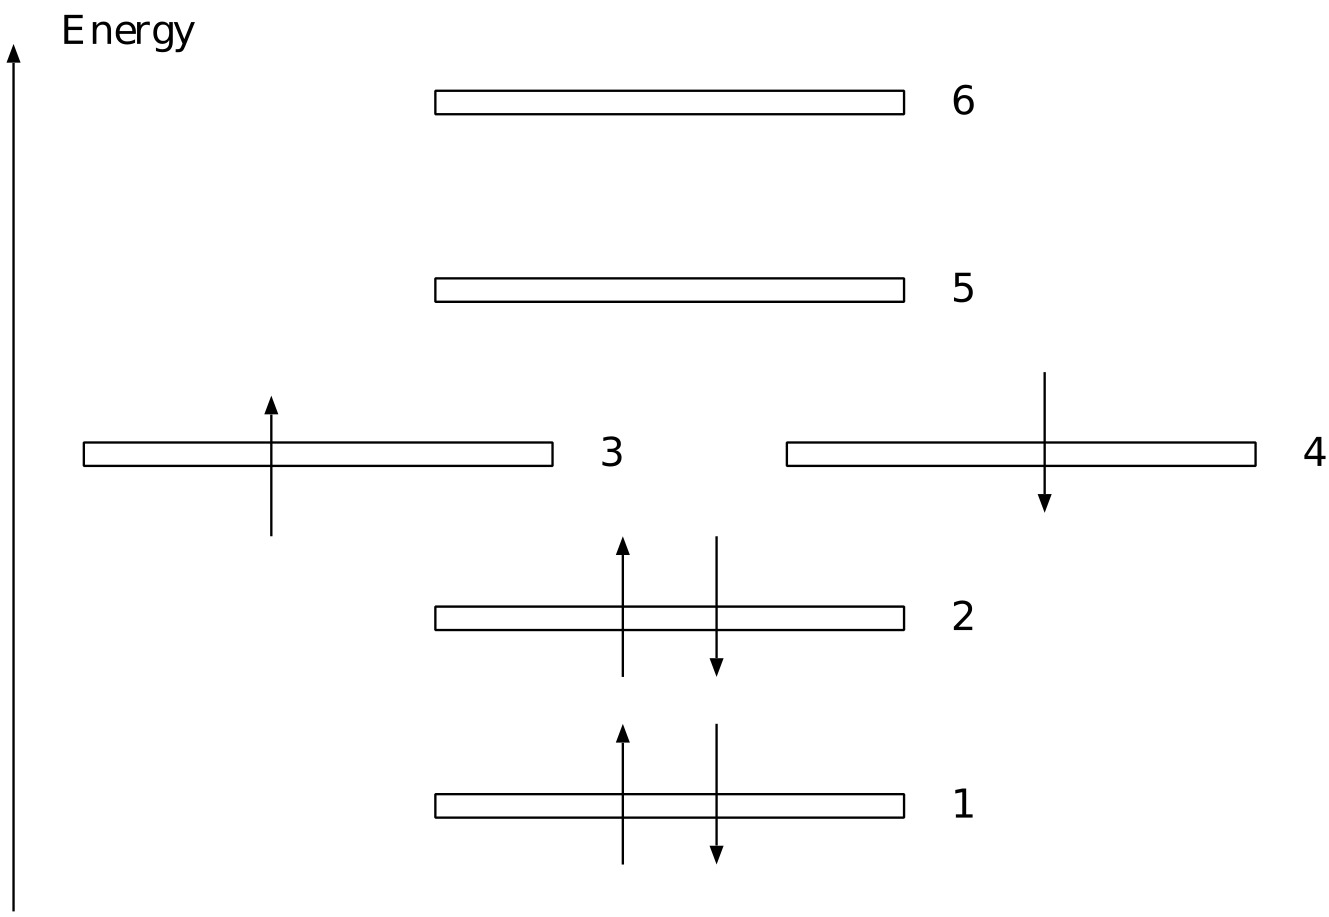
\includegraphics[width=60mm]{figures/CAS1}}
	\subfloat[Slater determinant $|1\bar{1}2\bar{2}3\bar{3}\rangle$]{\label{figure:2}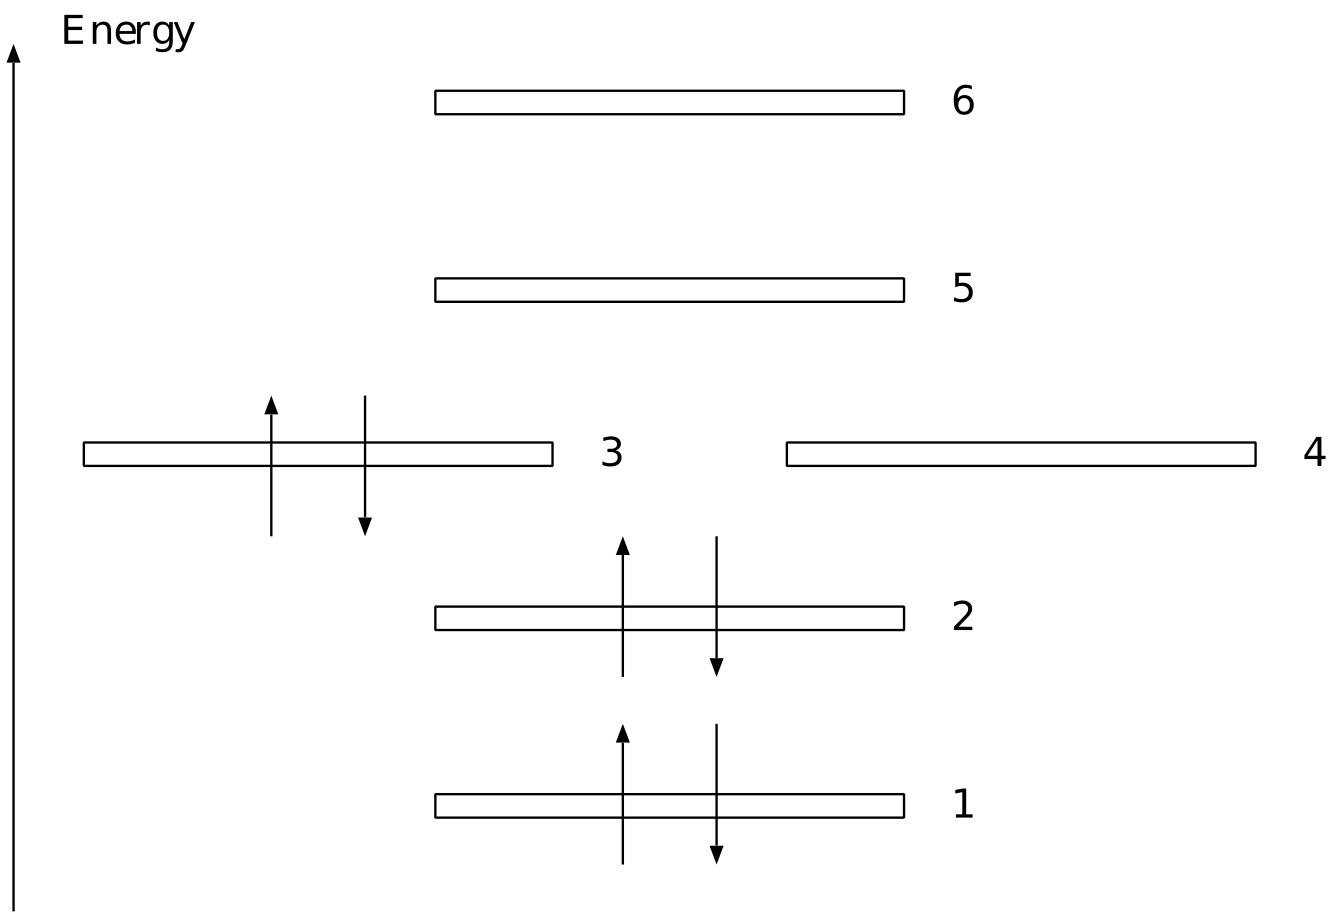
\includegraphics[width=60mm]{figures/CAS2}}
	\\
	\subfloat[Slater determinant $|1\bar{1}2\bar{2}\bar{3}4\rangle$]{\label{figure:3}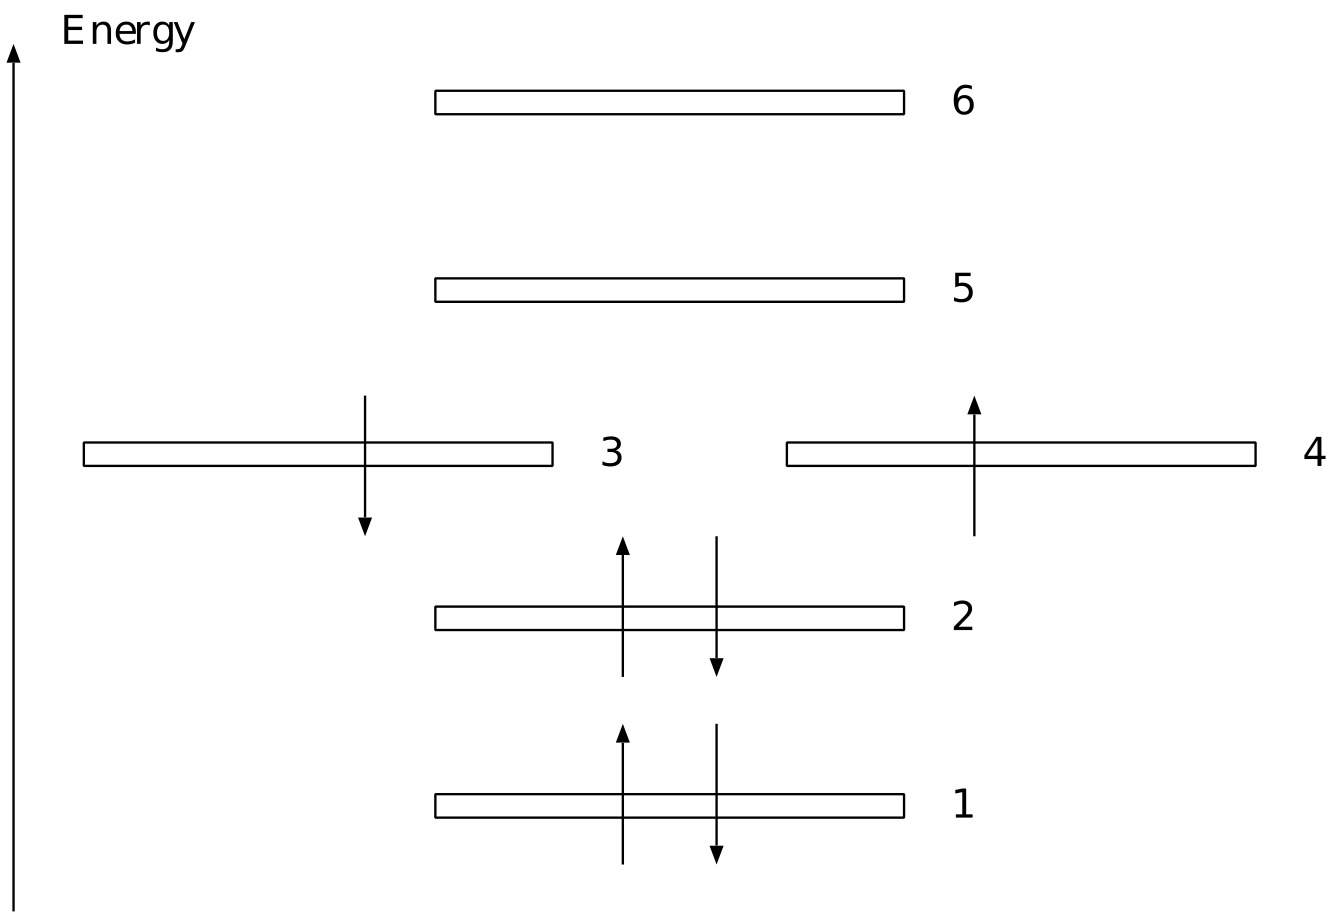
\includegraphics[width=60mm]{figures/CAS3}}
	\subfloat[Slater determinant $|1\bar{1}2\bar{2}4\bar{4}\rangle$]{\label{figure:4}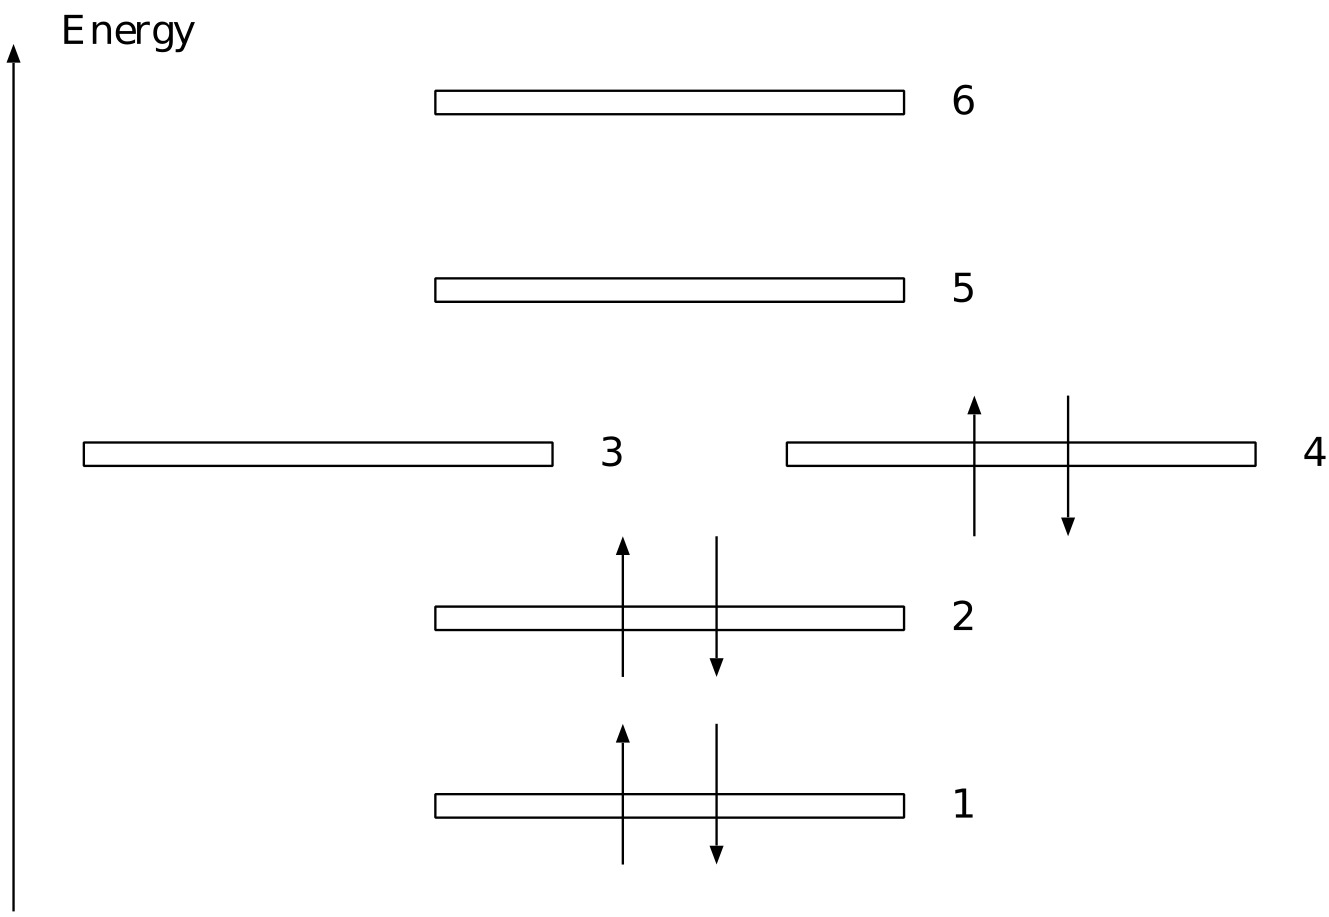
\includegraphics[width=60mm]{figures/CAS4}}
	\label{fig:CAS}
\end{figure}

\begin{figure}
	\centering
	\label{figure}
	\caption{Ground state from figure (1) + single excitation examples (many more exist; number of configurations scale exponentionally with electron population N)}
	\subfloat[Slater determinant $|1\bar{1}2\bar{2}3\bar{5}\rangle$]{\label{figure:5}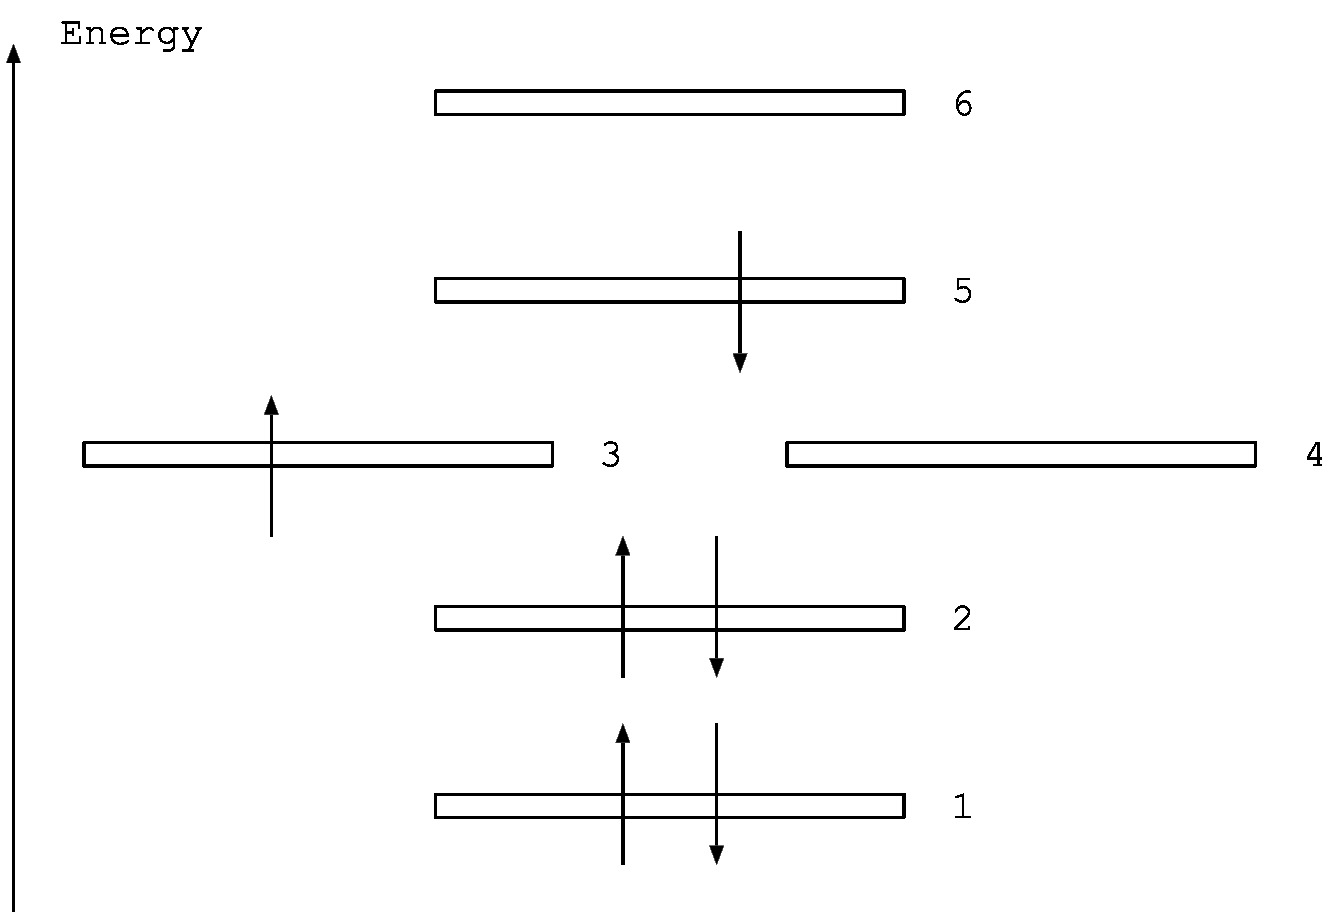
\includegraphics[width=60mm]{figures/CAS+S1}}
	\subfloat[Slater determinant $|1\bar{1}2\bar{2}\bar{4}6\rangle$]{\label{figure:6}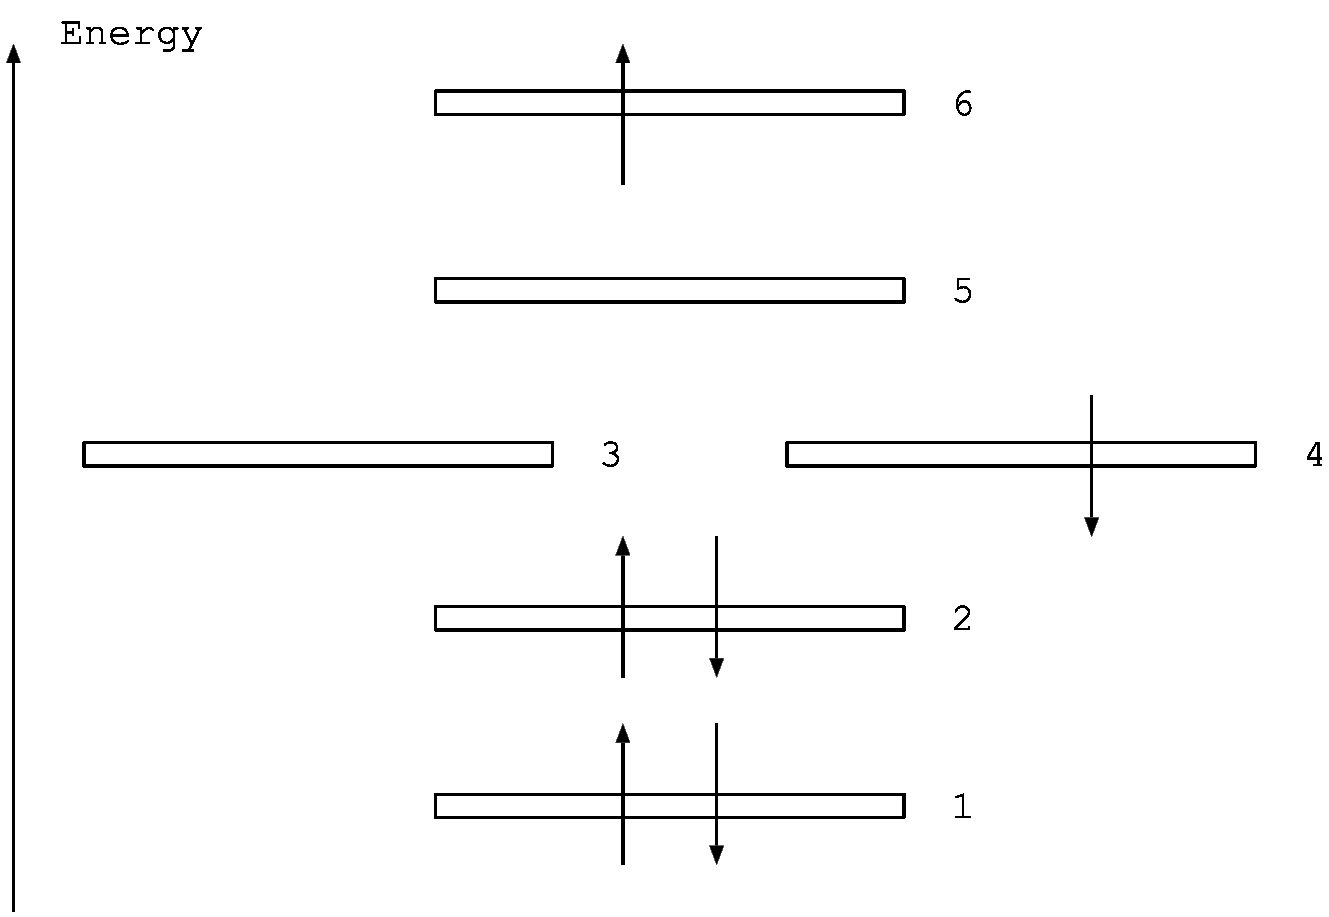
\includegraphics[width=60mm]{figures/CAS+S2}}
	\\
	\subfloat[Slater determinant $|1\bar{1}\bar{2}3\bar{4}5\rangle$]{\label{figure:7}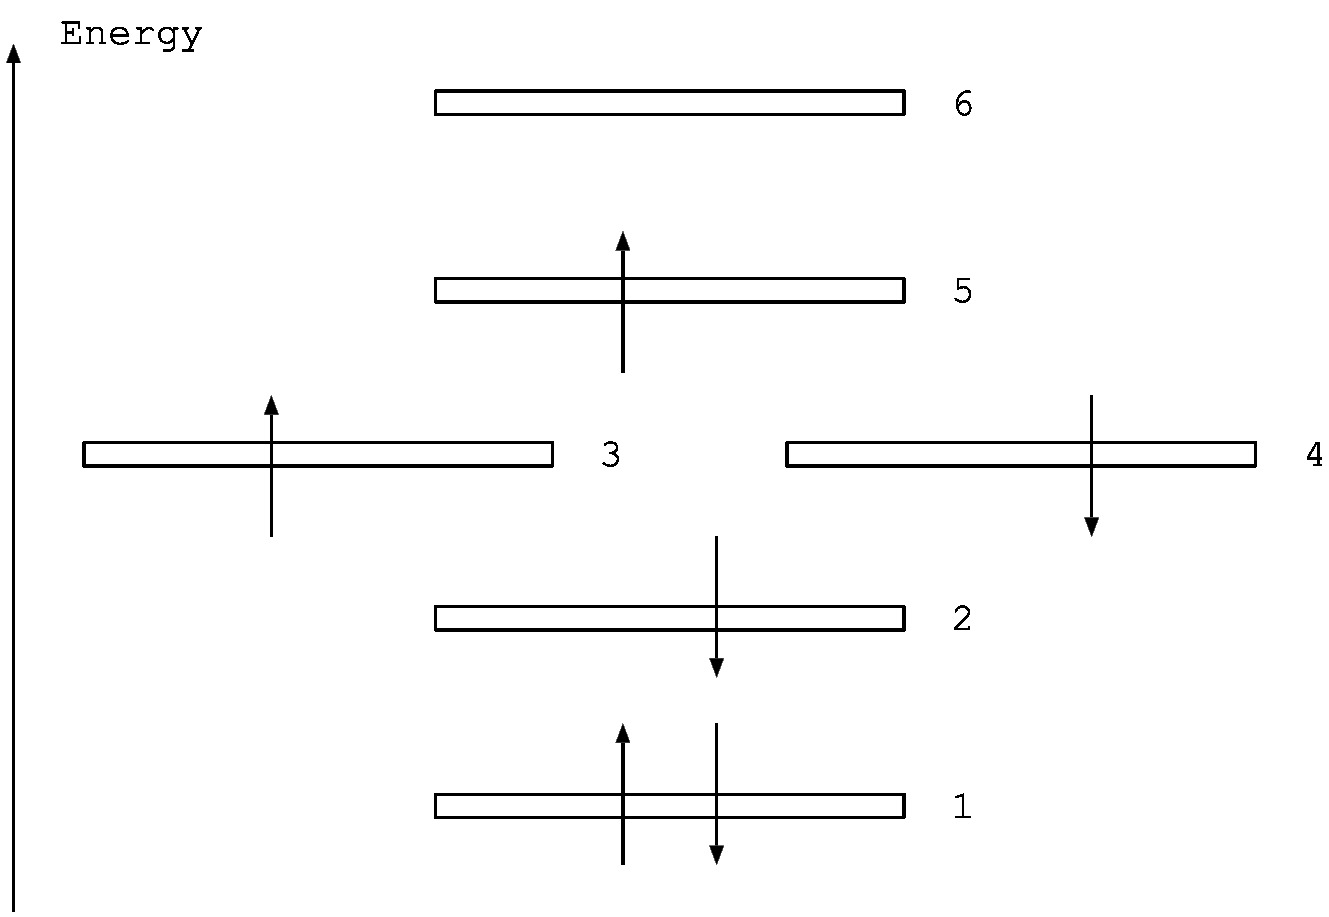
\includegraphics[width=60mm]{figures/CAS+S3}}
	\subfloat[Slater determinant $|12\bar{2}3\bar{4}\bar{6}\rangle$]{\label{figure:8}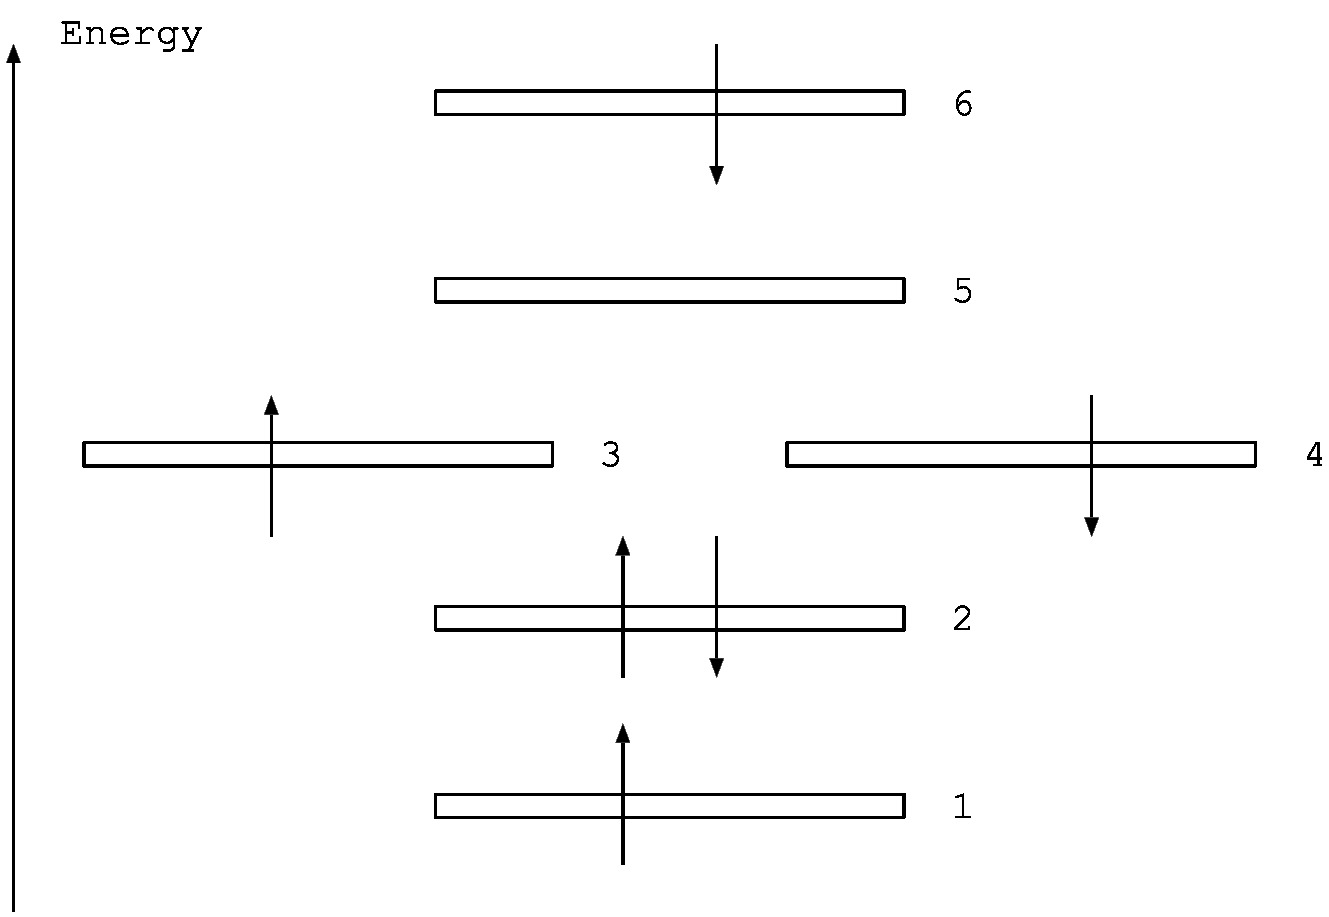
\includegraphics[width=60mm]{figures/CAS+S4}}
\end{figure}

In general, extended FCI models are very effective at accurately approximating these energies, but some discrepancies appear. An example is the CC3 cluster method which generates excellent agreement with regular-model FCI results when the excited states are dominated by a single excitation, but displays considerable error when faced with a large double-excitation character. Another example is the multi-reference method CASPT2, which gives very good results for a large number of systems, but significant errors appear when the reference SD space and outer SD space are not sharply separated.

DDCI solves these problems by building a configuration interaction with a small reference space, in the subspace of singles and doubles which contributes to the energy difference on the grounds of second-order perturbation considerations, i.e. a subspace defined by the `complete active space' (CAS) for all singles, and the doubles which involved at least one active orbital \cite{garcia1997application}. If faced with a system with numerous open-shells per atom (e.g high-spin manganese, cobalt, iron oxides), the computational cost of using CAS+DDCI or the LCAS+S (`large complete active space + single excitation' method) becomes prohibitive since the size of the space to diagonalise scales exponentially with the number of magnetic electrons. We can establish a simple physical criterion to select important reference configurations, and derive from it a novel method with a strongly reduced computational cost. This is because configurations involved LCAS+S for example, are far too numerous compared to the necessary methods for a good quality modelling of low-lying energy state physics. Something needs to change when approaching this type of problem.

\subsection{Modifications of the Standard WCMs and Effective Hamiltonian Criteria}

When solving this problem several modifications were made to the existing configuration methods by solid-state physicists. Compared to the LCAS+S, the multiple metal-to-metal and ligand-to-metal charge transfer configurations were removed from the reference part of the wavefunction (a ligand is an ion or molecule bound to a central metal atom; the charges being transferred are electrons between these bodies). When comparing to the CAS+DDCI, the multiple metal-to-metal charge transfer configurations and associated screening configurations were removed.

Additionally, double excitations were restricted to screening excitations on the ligand-to-metal charge transfers. This meant that the number of configurations in a magnetic interaction between two high-spin Mn III ions, for CAS+DDCI and LCAS+S, were reduced from approximately 10 billion and 60 billion, to 20 million, respectively. This less computationally expensive approach is called the `selected active space' method (SAS+S); see \cite{gelle2009accurate} for more on this approach. This optimised, embedded fragment, quantum chemical ab initio method allows for analysis of the local fluctuations of magnetic couplings in metal compounds like manganites, which were known to be influential in the macroscopic magneto-resistance effects but not accessible experimentally. This approach is mentioned because it is utilized in this project's simulation chain; it is important to generate a configuration approach calibrated to studying a certain property. In this case, SAS+S has the best accuracy to calculation time ratio for studying the magnetoelectric coupling of multiferroic materials.

After the system geometry optimisation in CRYSTAL, Env takes the positions of a chosen quantum fragment in the ground state and prepares it for embedding. The results are fed through a program called Env2Seward (see section 6). Then the MOLCAS chain (another ab initio computational chemistry program) handles the SAS+S method, enabling us to provide an adequate description of the electronic correlation interactions and leads us closer to discovering the magnetoelectric properties of the system.

%%%%%%% Here is wherre my understanding starts to become less than 100%

%With both methods a dynamical correlation correction on each reference determinant is included, independent of whether they are based on either the CAS or a zeroth-order multi-reference space retaining the dominant configurations for low-lying states. Highly accurate spectra are consequently obtained, from which effective-exchange integrals can be extracted using an effective Hamiltonian method. This is a Hamiltonian that acts in a reduced space and only describes a part of the eigenvalue spectrum of the true Hamiltonian. The Heisenberg Hamiltonian of equation (1) works on fictitious electron spin variables of magnetic subsystems, describing only low-lying energy states. However, these evaluations yield energy values within the error bar of experimental inelastic neutron scattering results.

%The ground and low-lying energy state eigenvalues and wavefunctions provided by these calculations are for a set of fragments designed to suit all the crystallographically independent effective interactions. One can use the described effective Hamiltonian theory to obtain a spin Hamiltonian separate from the Heisenberg one, that also works on fictitious effective electron variables but also nuclear spin variables. It typically only describes the $(2s+1)(2l+1)$ magnetic sublevels of the complete spectrum, where s and l are the spin and orbital angular momentum quantum numbers, respectively. \cite{mostafanejad2014basics}. The objective for the solutions of this spin Hamiltonian is that on each fragment it mimics the eigenvalues of the system that the fragment is embedded within, and that it's eigenvectors reproduce the main configurations of the ab-initio wavefunctions. The projection must be onto a subset of the zeroth-order multi-reference space chosen for the ab-initio calculation, as seen in this equation for the system wavefunction\cite{gelle2009accurate}:

%\begin{equation*}
%	|\psi_m\rangle = |\psi^0_m\rangle + |\psi^{ct}_m\rangle + |\psi^*_m\rangle
%\end{equation*}

%where $|\psi^0_m\rangle = \sum_{I}C^0_{I,m}|\Phi^0_I\rangle$, and $|\Phi^0_I\rangle$ represents the zeroth order CAS reference configuration. The coefficients for each determinant are found by diagonalising the effective Hamiltonian. This projection must represent at least $\sim90\%$ of the wave function of all involved states. Once the projection operator that accommodates these requirements is chosen, it is possible to achieve this in minimising the Lagrangian with respect to the fictional effective Hamiltonian variables:

%\begin{equation*}
%	\min_{J_{ij}} \mathcal{L}(J_{ij}) = \min_{J_{ij}} \sum_I ||\hat{H}(J_{ij})\hat{P}|\Psi_I\rangle-E_I\hat{P}|\Psi_I\rangle||^2
%\end{equation*}

%$\hat{H}(J_{ij})$ is the spin Hamiltonian, $|\Psi_I\rangle$ is the wave function for the $I$th excited state and $E_I$ its energy, and $\hat{P}$ is the aforementioned projection operator. The accuracy of this chosen $\hat{H}(J_{ij})$ is insured by the fact that $\sqrt{\mathcal{L}(J_{ij})} << J_{ij}$ and about $90\%$ of the \textit{ab initio} wavefunctions are represented for all fragments. 

\section{Calculation of the Displacement with CRYSTAL}
CRYSTAL is a program initially written by V.R. Saunders, R. Dovesi, C. Roetti and others from the Theoretical Chemistry Group at the University of Torino as well as the Daresbury Laboratory in Cheshire, England. It performs ab initio calculations of the ground state energy and the energy gradient of a condensed system. It also has the potential to generate the electron wavefunctions and consequently their behaviour in a periodic system. Hartree-Fock and Kohn-Sham Hamiltonians are typically used, employing postulates of DFT, to achieve these outcomes. Periodic systems are approximated by expansion of the single-particle wavefunctions as a linear combination of Bloch functions \cite{dovesi2017crystal17}.

A wave function that can be written as a plane wave modulated \footnote{Modulation is the varying of the properties of a periodic waveforml; an example is frequency modulation (FM) and amplitude modulation (AM) in radio systems} by a periodic function is a `Bloch wave', typically used to describe crystallographic electrons. Bloch functions are modulated by local functions or `Atomic Orbitals', which are linear `Gaussian type functions' used in the `Linear Combination of Atomic Orbitals' (LCAO) method. The various molecular symmetries (s, p, d, f, sp e.t.c) of the structure are used to modulate these LCAO orbitals \cite{dovesi2017crystal17}.

From a DFT calculation with CRYSTAL, after the optimal geometry is obtained with the execution keyword \verb|OPTGEOM|, we can print the Hessian matrix to file with the keyword \verb|PRINTHESS|, which is processed by the script discussed in section 6. The Born charges are printed automatically, and with the lattice parameter and unit cell data, we can begin to approach obtaining the atomic displacements for a given system, incident upon which is a chosen uniform electric field.


%\subsection{Calculation of the J}

%From a set of inputs for the software suite used for a point of the calculation
%\begin{itemize}
%	\item env15
%	\item seward
%	\item rasscf
%	\item localisation
%	\item matrec
%	\item kinorb
%	\item rasscf - ci only
%	\item motra
%	\item sass
%	\item prop
%\end{itemize}

\section{Solving the displacement equation}
\subsection{Generating the atomic displacements}

Once we have optimised the geometry of a system in CRYSTAL in order to minimise the total energy, i.e. finding the Hessian or minimum critical point of the $3N$ dimensional vector space, where $N$ is the number of atoms in the unit cell, we can generate the output files to be processed in order to solve the displacement of each atom for a given homogeneous electric field. 

\subsection{Details of Script Mechanisms}

\texttt{disp\_solve.py} is the second python driver script that I wrote at ILL. The script's first purpose is to parse the \texttt{.loto.out} or the \texttt{.DAT} output file from a CRYSTAL environment after the geometry of the system has been optimised and the consequential Hessian matrix and Born tensor have been calculated. The final output of the script is a grid of unit cell atomic coordinate files whose ions have been displaced by a range of uniform incident electric fields in various directions. The CRYSTAL output file(s) contains several pieces of information that are required for the next step towards this output.

Firstly, \texttt{disp\_solve.py} parses for and stores the total number of atoms in the unit cell for a system `$N$'. This gives us the first dimension of the Born and Hessian matrices ($3\times 3$ Cartesian-basis Hessian components $\mathcal{H}_{ij}$ or the diagonalised $3\times 3$ Born charge elements $q_{ij}$ for N atoms adds up to a total dimension of $3N$) so we can allocate the correct amount of space to append the parsed values to. Then the script parses for the aforementioned $N$ sets of $3\times3$ Born charge matrices and arranges them into the required diagonalised format. Lets say $a_{ij}$ is the matrix element of the ith row and the jth column, then the element with $i = j = 3n+1$, where $n \in \mathbb{Z}$ and bounded by $0 \leq n \leq N-1$, is the centre for the nth Born charge matrix. Any Born tensor element separated by an index of more than one from any of these centres is zero.

Once the Born tensor has been generated, the lower triangular symmetric Hessian from the \texttt{.loto.out} file is parsed for and mapped so that $a_{ij} \equiv a_{ji}$ for $i < j$ and it becomes square and symmetric across the diagonal. If the Hessian data is not contained within this file, there is a contingency to scan and symmetrise the \texttt{HESSIAN.DAT} file. For both of these matrices there is a small machine error from the CRYSTAL output that needs to be removed, so for every value $\leq 10^{-12}$ it is reduced to zero to minimise uncertainty. Once we have both formatted matrices (the Hessian $\mathcal{H}$ and Born tensor $q$) we can solve the force equation for displacements $d$ caused by an incident uniform electric field $E$ on the crystal that is chosen beforehand (recall equation (5)):
\begin{equation*}
q.E = -\mathcal{H}.d
\end{equation*}
using numerical python linear algebra modules (\texttt{numpy.linalg.solve}) that employs the Lapack routine \texttt{\_gesvx} written in Fortran. This equation will take place uniformly in Hartree atomic units in Cartesian coordinates as this is the output format from CRYSTAL.

\subsubsection{Conversion derivations}
In order to achieve this format for equation (5), we must convert the user's electric field inputs to Hartree field units.The electric field is entered into the above equation as $E_1, E_2, E_3$ in the $x, y, z$ Cartesian basis, in units of $kV/m$, to be converted to atomic units in the same basis. 

\begin{equation}
	(Ex, Ey, Ez) = conversion*(E_1, E_2, E_3)
\end{equation}

The electric atomic field conversion is given as:

$$\frac{E_h}{ea_0} = 5.142...\times 10^{11} (V/m)$$

where $E_h$ is the Hartree energy, $e$ is the unit electric charge and $a_0$ is the Bohr radius. To convert from $kV/m$ to these atomic field units, we must multiply our input values by $1000$ to obtain the same base SI units ($kV/m$ to $V/m$) as the atomic field units so that the conversion value is dimensionless, and then divide by $E_h/ea_0$:

$$\text{Input units to a.u. conversion} = \frac{kV/m}{E_h/ea_0} = \frac{1000(V/m)}{5.142...\times 10^{11} (V/m)} = 1.94...\times10^{-9}$$

%but when we need to divide by the lattice parameters, these are given in Angstrom from the crystal file data being used. Therefore an Angstrom to Bohr conversion must be included:

%$$\text{Total conversion} = \frac{kV/m}{E_h/ea_0}\times\frac{1}{\text{Angstrom to Bohr conv.}} = \frac{1000(V/m)}{5.142...\times 10^{11} (V/m)}\times \frac{1}{1.889725989}$$ 

%where ${E_h/ea_0}$ are the atomic field units given in terms of the Hartree energy. If this conversion is included in equation (10), the correct units will be obtained for the electric field vector to be used in equation (5).

If this conversion is included in equation (10), the correct units will be obtained for the electric field vector to be used in equation (5).
\\

% The below section is commented because the Hessian is actually given in Cartesian coordinates.

%Crystal provides the Hessian in fractional units, and so the matrix elements must be converted for the full equation to have uniform units. Since each element is a second derivative, the change between the output units as the units we need are generally derived as follows:

%Let $x$ be a length in one unit systems and $u$ a length in a different unit system. $x=C_{xu}\cdot u$ where $C_{xu}$ is the conversion factor between the two length scales. Taking derivative of a quantity $E$ with respect to $x$ we obtain:
%$$\frac{\partial E}{\partial x} = \frac{\partial E}{\partial u}\frac{\partial u}{\partial x} = \frac{1}{C_{xu}}\frac{\partial E}{\partial u}$$

%A similar method can be use to obtain the second derivative with respect to another coordinate, to a different unit scale ($y = C_{yv}v$):

%$$\frac{\partial^2 E}{\partial x \partial y} = \frac{1}{C_{xu}C_{yv}}\frac{\partial^2 E}{\partial u \partial v}$$

%In order to convert the Hessian from fractional units (Hartree energy $[E]$) to a.u. ($[E L^-2]$) we need to determine which index in the matrix includes (a,b), (a,c) or (b,c) in the denominator so we know what to divide by when converting ($C_{xu}$ and $C_{yv}$ in our more general example). This is because the three possible Hessian elements in a.u. are given as:

% Is this an ok notation for the Hessian elements?

%$$\frac{\partial^2E}{\partial(a_i/a)\partial(b_j/b)} \ \text{or} \ \frac{\partial^2E}{\partial(b_i/b)\partial(c_k/c)} \ \text{or} \ \frac{\partial^2E}{\partial(a_i/a)\partial(c_k/c)}$$

%If the Hessian matrix element of the ith row and jth column is given by $\mathcal{H}_{ij}$ then:
%$$\mathcal{H}_{11} \ \text{becomes} \ \mathcal{H}_{11}/a^2, \ \mathcal{H}_{12} \ \text{becomes} \ \mathcal{H}_{12}/ab, \ \mathcal{H}_{13} \ \text{becomes} \ \mathcal{H}_{13}/ac \ \text{e.t.c.}$$ 

%The division depends upon the modulus of the i or j index with 3: $mod(i,3) \ \text{or} \ i \ \% \ 3 = 0,1,2$ corresponds to a division by $a,b,c$ respectively. Then we need to discern what the proper conversion factor is when going from fractional units to atomic units. If we divide by the lattice vector lengths in Angstroms, we must include the square inverse of the Angstrom to a.u. conversion factor. This is not necessary if we divide by lattice vectors given in atomic units.

%This means the total conversion depends upon the matrix element's index but will always be divided by lattice parameters in Bohr units in the $a, b, c$ basis. The Born tensor is given in $e$ units in the a,b,c basis and so no conversion or transformation is required. Consequently, the displacements are output from the calculation as a $3N$ dimensional column vector in a.u. and converted to fractional units where $a_n/a, \ b_n/b,\ c_n/c = 3n,\ 3n+1,\ 3n+2$ for the nth atom ($0\leq n \leq N-1)$.

Once we have computed `$d$' for a given incident field in this format, the next step is to add the displacements to the unit cell file containing all of the relevant atomic coordinates. Before this is possible, it is necessary to convert to the displacements to fractional units in the crystallographic basis. This is the format of the cell files taken as input for Env15, and so our displacement basis and units must match. In order to make this conversion, we must parse the CRYSTAL \texttt{.loto.out} file for the basis conversion matrix ($x, y, z$ to $a, b , c$). Since this matrix is given in Angstrom units, the displacements must be converted from a.u. (Bohr) to Angstrom. Once the Bohr to Angstrom conversion has been applied, we can multiply our Cartesian displacements for each atom by this $3\times 3$ conversion matrix, and then divide the results by the corresponding lattice vector. See below for an example:
\\

Bohr to Angstrom conversion:

$$
	B2A = 0.529177210903
$$

Parsed basis conversion matrix in Angstrom:

$$
C = \begin{pmatrix}
C_{11} & C_{12} & C_{13} \\
C_{21} & C_{22} & C_{23} \\
C_{31} & C_{32} & C_{33}
\end{pmatrix}
$$

Cartesian coordinates for the nth atom:

$$d = \begin{pmatrix}
x_n \\
y_n \\
z_n
\end{pmatrix}$$

Combine these with the lattice vectors $a,b,c$ to obtain the displacements in the new basis and units:

$$d' = \begin{pmatrix}
a_n/a \\
b_n/b \\
c_n/c
\end{pmatrix} =
\begin{pmatrix}
1/a \\
1/b \\
1/c
\end{pmatrix}\cdot
\begin{pmatrix}
C_{11} & C_{12} & C_{13} \\
C_{21} & C_{22} & C_{23} \\
C_{31} & C_{32} & C_{33}
\end{pmatrix} \cdot
B2A \cdot
\begin{pmatrix}
x_n \\
y_n \\
z_n
\end{pmatrix}$$

Perform this action for all N sets of coordinates and the displacements can now be added to the unit cell.
\subsection{The Cell File}

The initial cell file is another output file of the CRYSTAL program that gives the position of the atoms in the unit cell in fractional coordinates alongside their corresponding charges. If all the required information is stored in this file, the \texttt{unit\_source} parameter `direct' can be called and all unit cell information is parsed from this file. Sometimes the cell file can be generated by CRYSTAL in a different spatial group, and so the number of coordinate sets in this file can be different to $N$. However, if \texttt{unit\_source} = auto, \texttt{disp\_solve} can scan this initial cell file for the charge magnitudes of each atom and reformulate the cell file by parsing the CRYSTAL output file for the unit cell coordinates and irreducible groups.

A new unit cell file is then written for the disturbed system containing double-precision floats with the associated converted displacements added. Entering \texttt{charge} instead of \texttt{auto} does the same thing but requires the user to enter the charge values for each irreducible atom group. We know which atom corresponds to the nth index and so we can merge the two sets of coordinates. This is then done on a large scale by specifying a range of electric fields in the $x,y,z$ directions. A grid of cell files specified by the $E_x,E_y,E_z$ inputs are generated and stored in a directory location reported by the command line, named after the specified ranges chosen for the incident field.

Another option to solve $q.E = -H.d$ would be directly employing the LAPACK Fortran drivers that specify to the type of matrix you are trying to process (in this case a symmetric semi-definite Hessian) which can save lots of processing time and generate increased accuracy. The trialled module was the symmetric system driver DSYEVX, that was ran in tandem with the python script using an executable batch file so that the displacement results could be compared. It was concluded that the numpy linear algebra framework was sufficient for the calculation purposes, and so the next step was to add calculated displacements to the atom coordinates from the CRYSTAL output files and process them with Env, before reformatting them with Env2Seward for different values of the electric field \footnote{Please see the appendix for an instruction manual that covers more detail how to use this software.}. This will be automated so that we can effectively calculate $\frac{\partial d}{\partial E}$ \footnote{See section 8 for more information on this process.} (recall step 5 of section 3). 



\section{Processing Env output into Seward}
Env2Seward is the first driver script that I wrote my time at ILL; it was created to process the output files from the Env15 program, \texttt{prefix.env.sew0} and \texttt{prefix.env.psd}, that contain the fragment, TIP and Madelung potential coordinates and basis sets (see \cite{varignon2013ab} as well as \cite{gelle2008fast} and the associated local tools manual). It operates by parsing the input files for the various atom types and ordering the atom's coordinate data into sets categorised by each homogeneous atom type. It writes their associated basis sets from either a default path or chosen library file, chosen and input by the user.

Coordinates are compared between the \texttt{sew0} and \texttt{psd} files to confirm the identity and atom-type of the coordinate set. The script is quite general, allowing for 3 different formats of atomic identification in the Env output files, including contingencies for a symmetric basis in the \texttt{psd} file and a system exit if the coordinates do not match between the two input files. The user is prompted intuitively for input of the basis set corresponding to each atom and the desired basis library, if no input file is passed on the command line. However, the script can be automated (if the user desired a conversion loop in a batch file), by calling it from command line with a separate input text file as a second argument, with the libraries and basis sets contained in in this input file. This command line input file can be generated automatically by the program through user input, or manually by the user. A third available format is the interactive Jupyter notebook that provides instructions in markdown alongside the python 3 cells.

Regardless of the input approach taken, the coordinates are organised into quantum fragment, ionic pseudopotential and Madelung potential categories in a way that is readable by the SEWARD input algorithm after being assigned to a certain atom type. See figure (3) for an excerpt of the fragment output.


\begin{figure}[htbp]
	\hspace*{-2.5cm}
	\begin{BVerbatim}[fontsize=\small]
	\&SEWARD
	Title
	Excerpt
	
	Expert
	Verbose
	
	*** Fragment ***************************************************
	Basis set
	Mn.ano-rcc.Roos.21s15p10d6f4g2h.6s4p3d1f0g.
	spherical
	Mn01       0.000000000000       0.000000000000       2.749761859316        Bohr
	Mn02       0.000000000000       0.000000000000      -2.749761859316        Bohr
	End of basis
	****
	Basis set
	O.ano-rcc.Roos.14s9p4d3f2g.4s3p1d0f
	spherical
	O203       2.231731397024      -0.875526023191       0.000000000000        Bohr
	O204      -2.231731397024       0.875526023191       0.000000000000        Bohr
	O305       2.118901193775      -1.064763543958      -5.367483621542        Bohr
	O306      -2.119040147228       1.064763543958      -5.367483621542        Bohr
	O407       1.412183935493       3.326902091439      -2.642519536557        Bohr
	O408       1.412183935493       3.326902091439       2.642519536557        Bohr
	O409      -1.412183935493      -3.326902091439       2.642519536557        Bohr
	O410      -1.412183935493      -3.326902091439      -2.642626886230        Bohr
	O311       2.118901193775      -1.064763543958       5.367483621542        Bohr
	O312      -2.119040147228       1.064763543958       5.367483621542        Bohr
	End of basis
	****
	\end{BVerbatim}
	\caption{Excerpt of fragment coordinates from env2seward output file generated for SEWARD input of the GdMn2O5 system. No specified library so the default is used.}
\end{figure}

Again, the appendix contains an instruction manual that goes into more depth about specifically how to use this software.

\section{Linking CRYSTAL output, Disp\_Solve, Env15 and Env2Seward}

As discussed before, the CRYSTAL optimised geometry output files contain the associated minimum energy Hessian and Born charge tensor data, alongside the unit cell atomic coordinates and lattice parameters. CRYSTAL also produces the unit cell coordinates alongside the atom's charges in a \textbf{cell file}. This data can be used to calculate the displacements from an induced uniform electric field using `disp\_solve`, and a grid of new cell files are generated with electrically disturbed positions, based on the initial cell file passed as an input or the coordinates found in the \texttt{.loto.out} output file \footnote{This is a summary of sections 5 and 6, see those for more details.}. 

Another program that I wrote for this project was \texttt{crys2seward.py}. Crys2Seward edits the xenv15 (the executable Fortran file for Env) \texttt{envin} or \texttt{env.in} input files so that the env15 program can take cell files of different displacements from the disp\_solve outputs. It does this by matching the number of atoms in the unit cell with the input cell file, changing the cell file taken as input from the initial cell file to each displaced cell file in the grid, and adding the displacements to the central magnetic atom coordinates. Xenv15 then produces a grid of output files named: 

\begin{itemize}
	\item \texttt{prefix.<field\_values>.env.sew0}
	\item \texttt{prefix.<field\_values>.env.psd}
\end{itemize}

These are the new input files passed to the Env2Seward program (the prefix corresponds to the simulated system). Crys2Seward modifies the Env2Seward input data so that the script processes every pair of \texttt{.psd} and \texttt{.sew0} files in the grid, so that each set of fragment coordinates can be categorised into a prefix.sew.in format, to be later input into SEWARD. Each file grid (cell files, env15 output files, sew.in files) is contained in a directory named after the electric field ranges and filetype.

The largest calculation time sink for this script is running xenv15 for each cell file; this gets exponentially more expensive as the number of atoms in the unit cell increases. Program performance was tested by running the program chain for several systems including YMnO3 and CuO, with Env2Seward and Disp\_Solve being tested on systems such as GdMn2O5 and TbMn2O5.

\newpage
\section*{Software Manual Appendix}
\documentclass[10pt]{article}
\usepackage[utf8]{inputenc}
\usepackage{amsmath}
\usepackage{amsfonts}
\usepackage{amssymb}
\usepackage{hyperref}
\usepackage{courier}
\usepackage{graphicx}
\usepackage{listings}
\usepackage{color}

\definecolor{dkgreen}{rgb}{0,0.6,0}
\definecolor{gray}{rgb}{0.5,0.5,0.5}
\definecolor{mauve}{rgb}{0.58,0,0.82}

\lstset{frame=tb,
	language=Python,
	aboveskip=3mm,
	belowskip=3mm,
	showstringspaces=false,
	columns=flexible,
	basicstyle={\small\ttfamily},
	numbers=none,
	numberstyle=\tiny\color{gray},
	keywordstyle=\color{blue},
	commentstyle=\color{dkgreen},
	stringstyle=\color{mauve},
	breaklines=true,
	breakatwhitespace=true,
	tabsize=3
}

\author{Joshua Horswill}
\title{Env2Seward Technical Manual}

\begin{document}
\maketitle
\tableofcontents

\section{Author and Permissions}
This code was written by {\bf Joshua Horswill} during an internship with the ILL theory group in June 2020 under supervision of {\bf Marie-Bernadette Lepetit}. 
\\

It is permissible to use and diffuse this code provided J. Horswill and MB lepetit are kept informed. Modifications to this code can be made provided that the developer sends modifications to J. Horswill or M.B. Lepetit, so they may be included in the source code.
\\
\\

\hspace*{3cm}                
\begin{minipage}{10cm}
	MB Lepetit \\
	Institut Néel, CNRS UPR~2940 \\                       
	25 rue des Martyrs, BP 166, Bât. K\\
	38042 Grenoble cedex 9 \\
	FRANCE \\[+1ex]                                          
	{\bf Courriel :} Marie-Bernadette.Lepetit@Neel.CNRS.fr  \\
	
	J. Horswill \\
	Institut Laue-Langevin\\            
	71 Avenue des Martyrs,\\  
	38000 Grenoble,\\
	France\\[+1ex]                                          
	{\bf Email :} horswill@imap.ill.fr  \\
\end{minipage}
\section{Manual}
\subsection{Introduction}
As you may have guessed from the name of the script, this code processes and formats the output from a program called ENV so it can be used in a calculation performed by a program called SEWARD. These simulation scripts are found in the local tools manual for the `Fast calculation of the electrostatic potential in ionic crystals by direct summation method' written by MB Lepetit and A. Gellé. This local tools manual contains scripts that provide a ``set of charges that allow the calculation of the Madelung potential of an ionic crystal within a predefined accuracy" \cite{gelle2008fast}. This is designed for the purpose of performing an ab-initio quantum calculation on a `quantum fragment' that is surrounded by a first shell of ionic pseudo-potentials, and a second layer of renormalised point charges \cite{varignon2013ab}. The `prefix' is a placeholder for the name of the compound being simulated.

\subsubsection{How to compile and run the script}
A {\bf python 3} distribution such as `Anaconda' or `Active Python' must be downloaded, which provides the option of using integrated development environments (IDE) for programming in the python language. For the development of this script, `Spyder' was used. This is an IDE available in Anaconda. Before running the file, make sure the script is in the same directory as the input files described below. After you have made sure this is the case, open the file with an IDE (typically an 'open file' option in the top left of the window, or you can drag it into the IDE text editor), hit run, and answer the prompts in the terminal. If you want to install python directly, see \url{https://realpython.com/installing-python/}. Typing `\texttt{python3 env2seward.py}' in the terminal running in the same directory as the python file should execute the script, generating the prompts in the command line. The new file will appear in the same directory as the python script.
\subsection{Prompt entry}
\subsubsection{Inputs and outputs}
Prefix.env.sew0 is a help file that contains the input data for SEWARD of the MOLCAS chain. It contains the data for the quantum fragment, the TIPS and the renormalised charges. This is one of two input files for the env2seward script. The second is called prefix.psd, and contains the information on the atoms represented by TIPs. The ordering seen in this file is as follows: first, atoms that are irreducable (with symmetry), and second, all atoms (without symmetry). It also requires two groups of basis sets - one for the quantum fragment and one for the ionic pseudopotential. Once these have been prompted and entered through the terminal command line, an output file ready to be fed into SEWARD will be generated. This can be called prefix.sew.in.

In summary the files and data required for this program are:
\begin{itemize}
	\item \texttt{prefix.env.sew0}
	\item \texttt{prefix.env.psd}
	\item Fragment basis sets and library locations.
	\item Pseudopotential basis sets and library locations.
	\item Name of the prefix.
\end{itemize}
The input files must be in the same directory as the env2seward script for the program to run successfully. The first prompt before basis set and library input will be to ask if you are running the script in a Jupyter Notebook (see relevant section below). If you wish to be prompted for input, enter `N' or `n'. 

\subsubsection{Prefix, Title and Basis Set Formatting}

The prefix entered can be anything you want, but it must match the prefix on the input files. For example, if the prefix was `example', this automatically generates a seward input file called `\texttt{example.sew.in}'. However, this will not work unless the env input files have the filenames `\texttt{example.env.sew0}' and `\texttt{example.env.psd}'. The input on the prompt for the title will be written to the document introduction, and this does not depend on the name of the input files or the prefix.

Basis sets for the fragment potential are unique to the system being evaluated and so cannot be managed by env2seward. These must be entered individually when prompted by the command line, as well as their library location. For example, if oxygen is one of the elements contained within the input files, the command will prompt for it's basis set input after parsing the prefix.env.sew0 file. It will then ask for the specified library location. If the corresponding library is default for the system, leave the input blank and press enter. If this is not the case, submit the name of the specified library.
\\
It is almost the same for the pseudopotential, but the pseudo basis sets depend upon the charge of the atom. For example, for GdMn2O5 there are three elements but eight basis sets, since there are two types of gadolinium and manganese and four types of oxygen. This results in more prompts for the corresponding basis sets and libraries. The command line will distinguish between the inputs between the fragment and the TIPs. Continue until all basis sets have been entered and the file will be written.

\subsection{Reading Filenames, Basis Sets and Libraries from an Input File}

There is another option for entering the data required to format the ENV output files, and this is to write the filenames, title and basis set information in a text file. To do this, write the text file in the following format (each bullet point is a new line, although the order does not matter):

\begin{itemize}
	\item \texttt{filename = chosen\_filename}
	\item \texttt{title = chosen\_title}
	\item \texttt{sew0\_file = prefix.env.sew0}
	\item \texttt{psd\_file = prefix.env.psd}
	\item \texttt{lib\_frag = \{"atom\_type":\{"loc":"specified basis set library","key":"basis set for atom\_type"\},"atom\_type2":...\}}
	\item \texttt{lib\_pseudo = \{"atom\_type":\{"loc":"specified basis set library","key":"basis set for atom\_type"\},"atom\_type2":...\}}
\end{itemize}

The format of the basis set libraries is in the python dictionary syntax. This means each dictionary key (e.g \texttt{"atom\_type},\texttt{"loc"} and \texttt{"key"}) corresponds to a piece of data. In this case the data is either a string or another dictionary. Each atom is assigned to it's own dictionary containing a key for the specified basis set library (set to \texttt{"loc":""} if default) and a key for the basis set (\texttt{"key":"basis set"}).
Here is an example for a GdMn2O5 input file, where the fragment dictionary (\texttt{lib\_frag}) has no specified library but the TIP dictionary (\texttt{lib\_pseudo}) basis sets are found in PSEUDO:

\begin{lstlisting}
	filename = example.sew.in
	title = example
	sew0_file = GdMn2O5_J1.env.sew0
	psd_file = GdMn2O5_J1.env.psd
	lib_frag = {'Mn':{'loc':'','key':'Mn.ano-rcc.Roos.21s15p10d6f4g2h.6s4p3d1f0g.'},
	'O':{'loc':'','key':'O.ano-rcc.Roos.14s9p4d3f2g.4s3p1d0f'}}
	lib_pseudo = {'Gd1':{'loc':'PSEUDO','key':'Gd.ECP.Marie.0s.0s.0e-Gd1-GdMn2O5.'},
	'Gd2':{'loc':'PSEUDO','key':'Gd.ECP.Marie.0s.0s.0e-Gd2-GdMn2O5.'},
	'Mn1':{'loc':'PSEUDO','key':'Mn.ECP.Marie.0s.0s.0e-Mn1-GdMn2O5.'},
	'Mn2':{'loc':'PSEUDO','key':'Mn.ECP.Marie.0s.0s.0e-Mn2-GdMn2O5.'},
	'O1':{'loc':'PSEUDO','key':'O.ECP.Marie.0s.0s.0e-O1-GdMn2O5.'},
	'O2':{'loc':'PSEUDO','key':'O.ECP.Marie.0s.0s.0e-O2-GdMn2O5.'},
	'O3':{'loc':'PSEUDO','key':'O.ECP.Marie.0s.0s.0e-O3-GdMn2O5.'},
	'O4':{'loc':'PSEUDO','key':'O.ECP.Marie.0s.0s.0e-O4-GdMn2O5.'}}
\end{lstlisting}
Make sure that all variables are on the {\bf same line} as the string/dictionary they are being assigned to. There also must be spacing between the variable, the $=$ sign and the data, so that the parsing algorithm can identify the data and write it to the output file.

Make sure this file is in the same directory as the python script and the ENV input files. Once you have written this text file with the correct formatting and wish for it to be parsed by env2seward.py, enter the following command:

\begin{itemize}
	\item \texttt{python3 env2seward.py chosen\_input\_filename}
\end{itemize}

If the setup has been performed correctly, the script will output `File has been created' and the sew.in file will appear in the script directory.

\subsection{Jupyter Notebook Version}
To install Jupyter Notebook, follow this guide: \url{https://jupyter.org/install}. For the creation of the \texttt{env2seward\_notebook.ipynb} file, the Anaconda distribution was used to install Jupyter Notebook with the \texttt{conda} command. This is the recommended method (see \url{https://www.anaconda.com/products/individual} for distribution download). 
\\
Once you have installed Jupyter notebook you need to download and localise the following files into the same directory/folder:

\begin{itemize}
	\item \texttt{env2seward.py}
	\item \texttt{env2seward\_notebook.ipynb}
	\item \texttt{prefix.env.sew0}
	\item \texttt{prefix.env.psd}
\end{itemize}
Next we need to open the Jupyter Notebook web app. We can do this by:

\begin{itemize}
	\item Opening up a terminal in the directory containing the four files mentioned above.
	\item Entering `\texttt{jupyter notebook}' to initialise the web app.
	\item Your browser should open it in a new tab and you should see these four files in your notebook directory.
	\item Now open the \texttt{env2seward\_notebook.ipynb} file from the web app dashboard menu.
\end{itemize}

You should see the menu shown in figure (1) and the notebook shown in figure (2). In the notebook you will see a page of Jupyter cells, some in markdown (a text formatting language) and some to run python3 code. If you want to learn more about how these work, see \url{https://www.dataquest.io/blog/jupyter-notebook-tutorial/}. In order to run these cells individually, click on them and hit \texttt{Ctrl+Enter} or press the run button (below the cell tab in the toolbar). 
Please follow the instructions in between the code cells to enter the correct inputs. If you would like to see the atom-types that require basis set entry, follow the instructions under the subtitle `Basis atoms (see instructions below on how to run this cell):'. The next steps are:

\begin{figure}
	\centering
	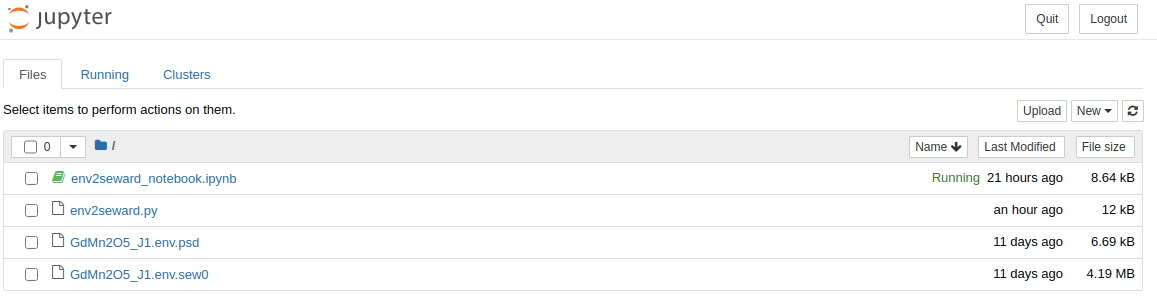
\includegraphics[width=1.3\linewidth]{dashboard.png}
	\caption{Web app dashboard menu}
	\label{fig:screenshot-from-2020-06-23-12-26-13}
\end{figure}

\begin{figure}
	\centering
	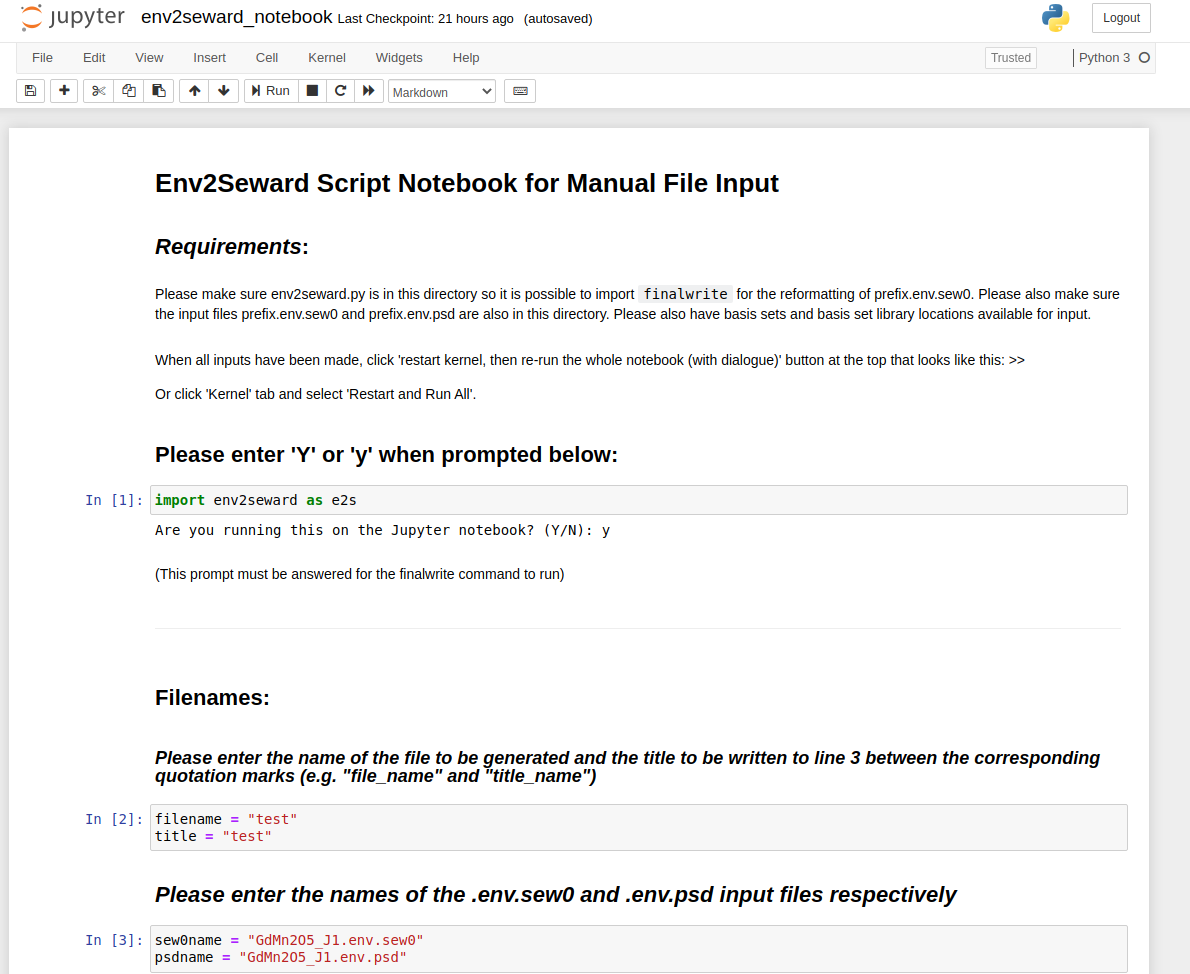
\includegraphics[width=1.3\linewidth]{notebook.png}
	\caption{env2seward\_notebook when opened}
	\label{fig:screenshot-from-2020-06-23-12-26-25}
\end{figure}



\begin{itemize}
	\item Make sure the inputs have all been entered according to the instructions (filename, title, sew0name, psdname, lib\_frag, lib\_pseudo)
	\item Select the button that says `restart the kernel and re-run the whole notebook' that looks like a fast-forward icon.
	\item If you cannot find this, click the kernel icon (in English, it may be different in other languages), next to cell and widgets, and select `Restart and Run All'.
	\item You will see a prompt in the first code cell (\texttt{import env2seward as e2s}). Please enter `Y'.
	\item After this the last code cell (\texttt{e2s.finalwrite(filename,...}) will output `File has been created' which means you now have a seward input file ready in the webapp directory. You can download this to a specific directory by going back to the dashboard menu, ticking the box next to `\texttt{chosen filename}' and clicking `Download'.
	\item The output file will also naturally appear in the same directory as your \texttt{env2seward\_notebook.ipynb} file.
\end{itemize}

\bibliographystyle{unsrt}
\bibliography{manualbib.bib}
\end{document}


\bibliography{reportbib.bib}
\bibliographystyle{plainurl}
\end{document}
